\section{Resultados}

\subsection{Envio e Recebimento de dados via Iperf3}

Para esta simulação, foi realizada a transmissão de um arquivo FTP e de um arquivo de voz. Para 
isso foi utilizada a ferramenta Iperf3, com o Host Zabbix atuando como servidor e o Host Linux como cliente. 
O teste de largura de banda entre os hosts foi realizado utilizando o protocolo TCP.

Na primeira simulação, foi realizada a transmissão de um arquivo FTP do Host Linux para o Host Zabbix. Na Figura \ref{fig:iperf2},
 é possível observar o comando utilizado para iniciar o servidor Iperf3 no Host Zabbix, 
 bem como o resultado do teste de largura de banda entre os dois hosts. 
 O teste indicou uma largura de banda de 1 Gbps,
  demonstrando a capacidade da rede para suportar a transferência de arquivos FTP de forma eficiente.


\begin{figure}[H]
    \centering
    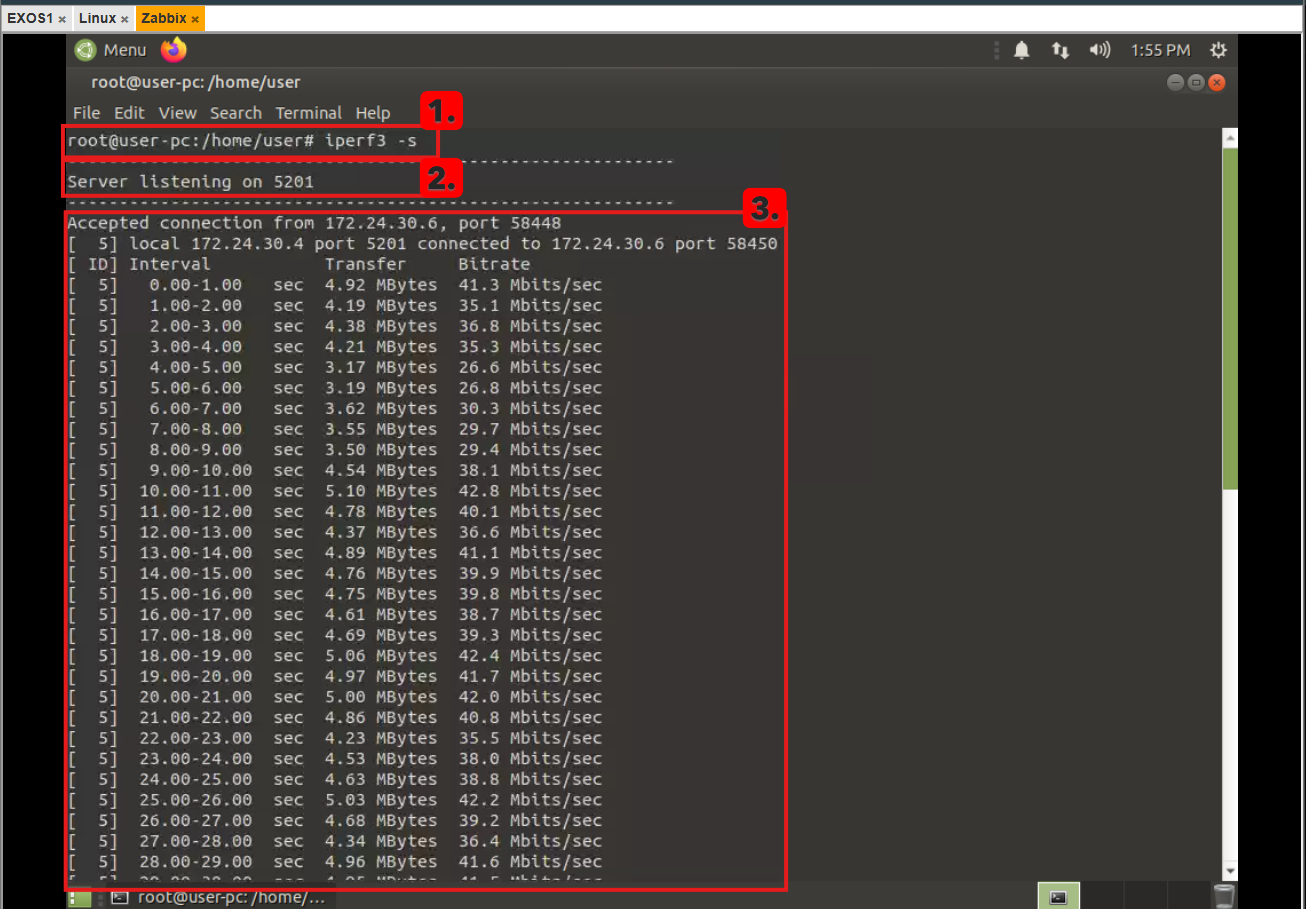
\includegraphics[width=1\linewidth]{fig/iperf2.png}
    \caption{Host Zabbix como servidor Iperf3 - transmissão arquivo FTP; 1. Comando para iniciar o servidor Iperf3; 
    2. Resultado do teste de largura de banda entre o Host Zabbix e o Host Cliente}
    \label{fig:iperf2}
\end{figure}

Na Figura \ref{fig:iperf1}, é possível observar o comando, \textit{iperf3 -c 172.24.30.4 -i 10 -p 5201 -w 8.0K -t 60},
utilizado para iniciar o cliente Iperf3 no Host Linux. O \textit{-c} especifica o endereço IP do servidor, 
\textit{-i} define o intervalo de tempo para exibir os resultados, 
\textit{-p} indica a porta utilizada para a comunicação, 
\textit{-w} define o tamanho da janela TCP e 
\textit{-t} especifica a duração do teste em segundos.

  
Ainda na Figura \ref{fig:iperf1}, é possível ver o resultado do teste de largura de banda entre o Host Linux e o Host Zabbix. 
O teste indicou uma largura de banda de 1 Gbps, confirmando a capacidade da rede para suportar a
transferência de arquivos FTP de forma eficiente.

\begin{figure}[H]
    \centering
    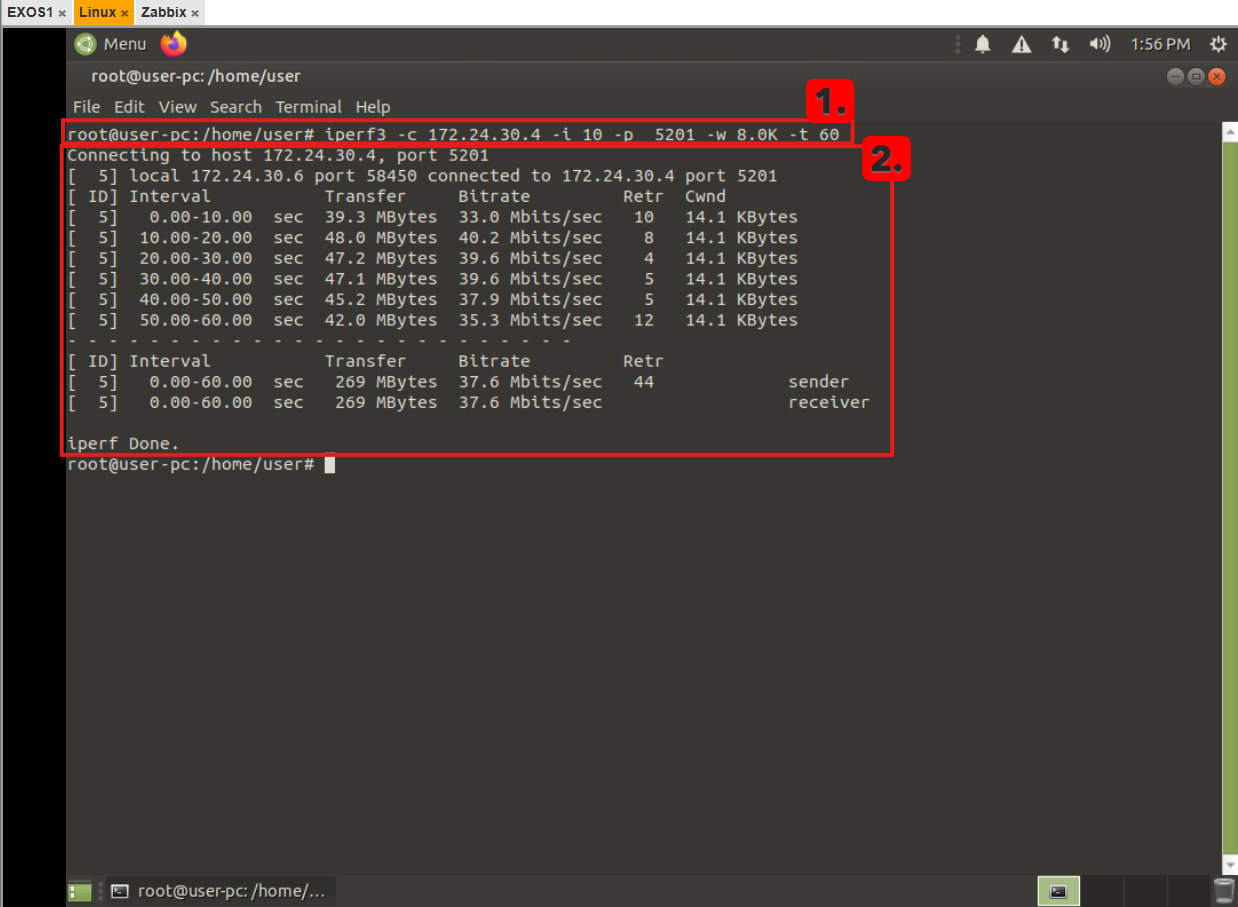
\includegraphics[width=1\linewidth]{fig/iperf1.png}
    \caption{Host Linux como cliente Iperf3 - transmissão arquivo FTP; 1. Comando para iniciar o cliente Iperf3; 
    2. Resultado do teste de largura de banda entre o Host Linux e o Host Zabbix}
    \label{fig:iperf1}
\end{figure}

Já na segunda simulação, foi realizada a transmissão de um arquivo de voz do Host Linux para o Host Zabbix.
Na Figura \ref{fig:iperf3}, é possível observar o comando utilizado para iniciar o servidor Iperf3 no Host Zabbix,
bem como o resultado do teste de largura de banda entre os dois hosts.

\begin{figure}[H]
    \centering
    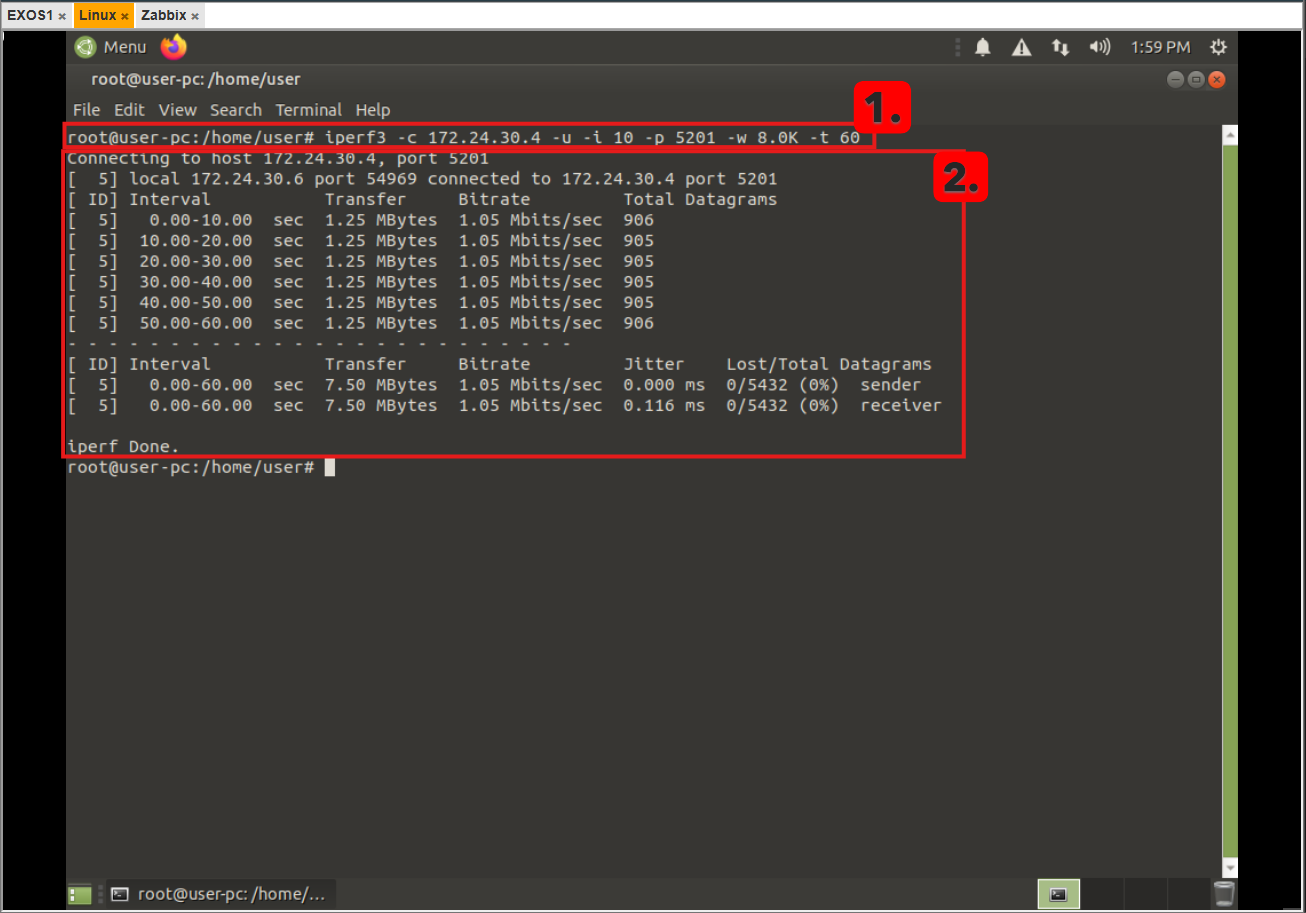
\includegraphics[width=1\linewidth]{fig/iperf3.png}
    \caption{Host Zabbix como servidor Iperf3 - transmissão arquivo de Voz; 1. Comando para iniciar o servidor Iperf3; 
    2. Resultado do teste de largura de banda entre o Host Zabbix e o Host Cliente}
    \label{fig:iperf3}
\end{figure}

Na Figura \ref{fig:iperf4}, é possível observar o comando,\textit{iperf3 -c 172.24.30.4 -u -i 10 -p 5201 -w 8.0K -t 60},
utilizado para iniciar o cliente Iperf3 no Host Linux. No comando, o \textit{-c} especifica o endereço IP do servidor,
O \textit{-u} especifica que o teste deve ser realizado utilizando o protocolo UDP, 
\textit{-i} define o intervalo de tempo para exibir os resultados,
\textit{-p} indica a porta utilizada para a comunicação, 
\textit{-w} define o tamanho da janela TCP e \textit{-t} especifica a duração do teste em segundos.    

Ainda na Figura \ref{fig:iperf4}, é possível ver o resultado do teste de largura de banda entre os dois hosts. O teste indicou uma largura de banda de 1 Gbps,
 demonstrando a capacidade da rede para suportar a transferência de arquivos de voz de forma eficiente.

\begin{figure}[H]
    \centering
    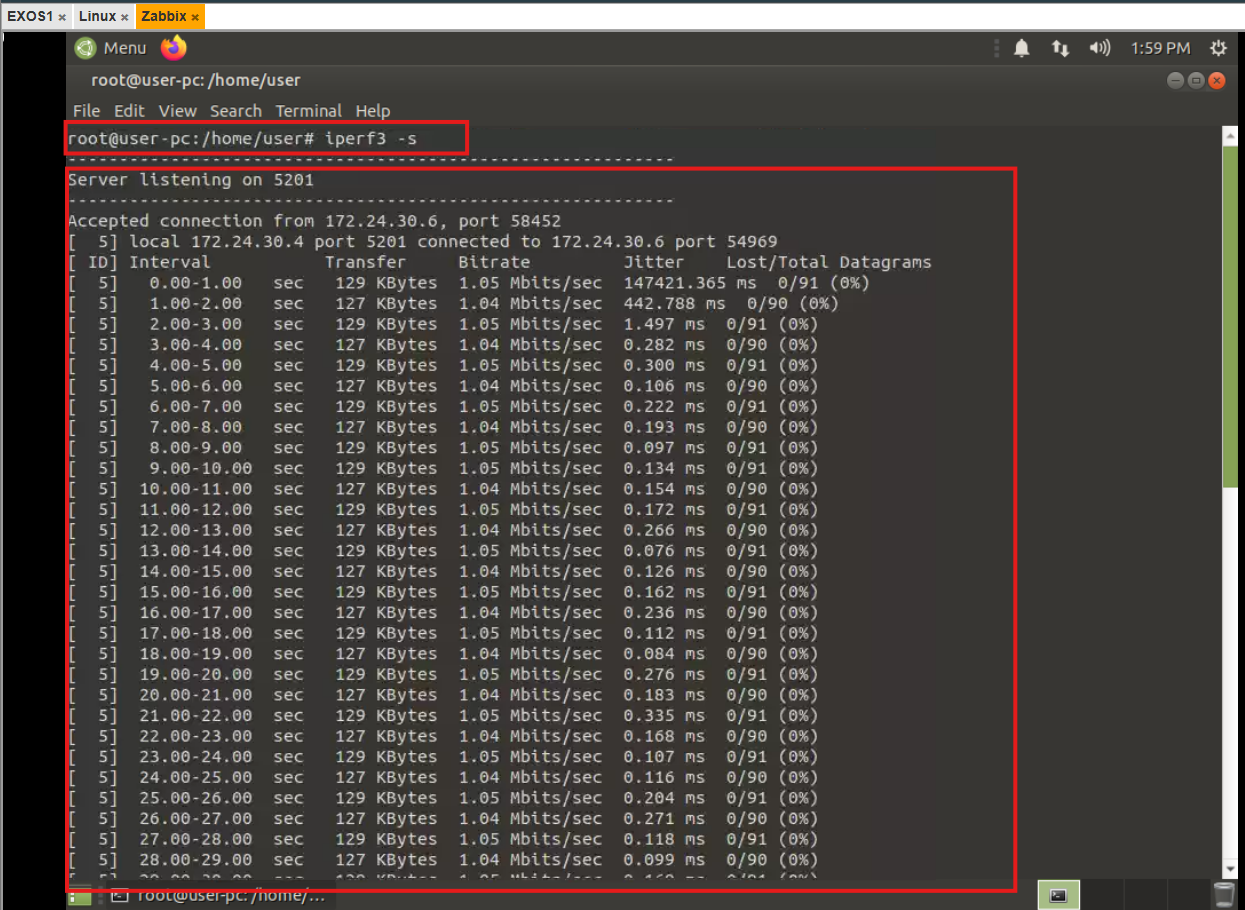
\includegraphics[width=1\linewidth]{fig/iperf4.png}
    \caption{Host Linux como cliente Iperf3 - transmissão arquivo de Voz; 1. Comando para iniciar o cliente Iperf3; 
    2. Resultado do teste de largura de banda entre o Host Linux e o Host Zabbix}
    \label{fig:iperf4}
\end{figure}

\subsection{NMAP}
Para a realização de testes de varredura de portas e identificação de serviços, 
foi utilizada a ferramenta Nmap, como mostrado na Figura \ref{fig:nmap1}. Foi utilizado 
o comando \textit{nmap 172.24.30.4}, que realiza uma varredura de portas 
no endereço IP do Host Zabbix. O resultado da varredura indicou 
que as portas 22 (SSH), 80 (HTTP) e 3306 (MySQL) estavam abertas, indicando a presença desses serviços no Host Zabbix.

\begin{figure}[H]
    \centering
    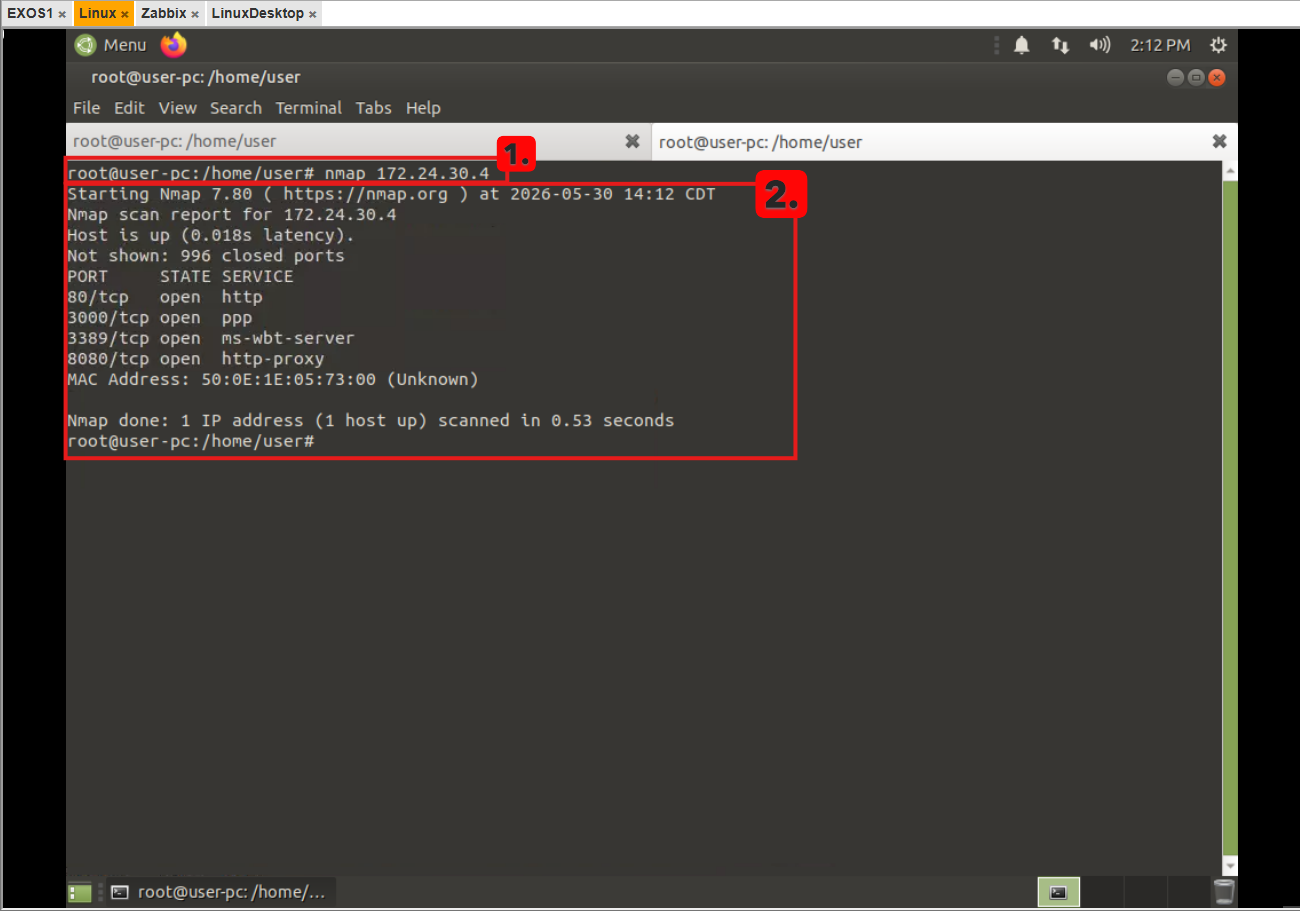
\includegraphics[width=1\linewidth]{fig/nmap1.png}
    \caption{Varredura de portas utilizando o Nmap; 1. Comando para realizar a varredura de portas no Host Zabbix; 
    2. Resultado da varredura indicando as portas abertas e os serviços correspondentes}
    \label{fig:nmap1}
\end{figure}


Já na Figura \ref{fig:nmap2}, foi utilizado o comando, 
\textit{nmap 172.24.30.4 172.24.30.254}, que realiza uma varredura de portas 
nos endereços IPs 172.24.30.4 e 172.24.30.254, 
o resultado da varredura indicou que as portas
22 (SSH), 80 (HTTP) e 3306 (MySQL) estavam abertas no Host Zabbix, 
enquanto as portas dos outros hosts estavam fechadas, indicando a 
ausência desses serviços nos demais hosts da rede.

\begin{figure}[H]
    \centering
    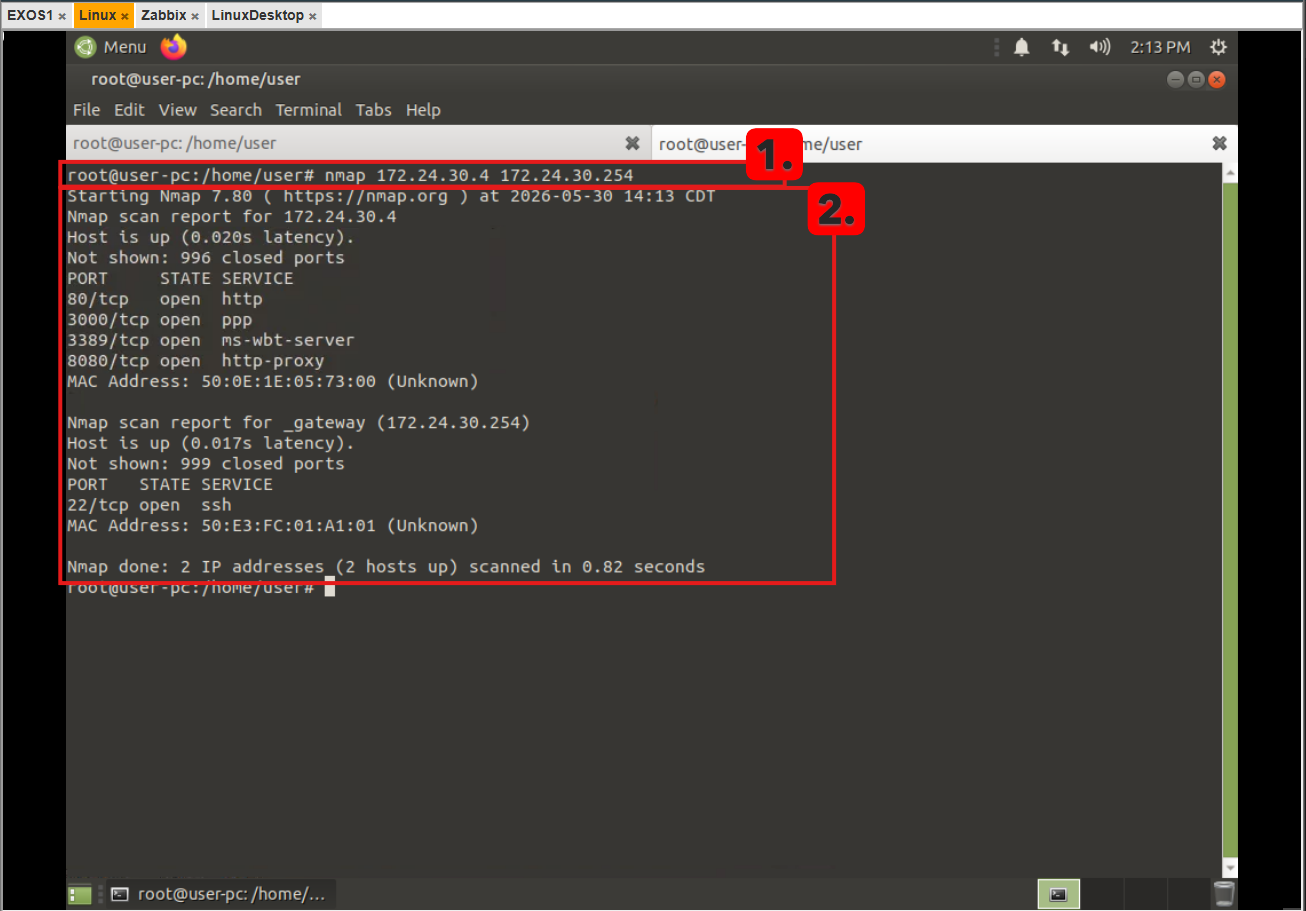
\includegraphics[width=1\linewidth]{fig/nmap2.png}
    \caption{Varredura de portas utilizando o Nmap; 
    1. Comando para realizar a varredura de portas nos endereços IPs 172.24.30.4 e 172.24.30.254; 
    2. Resultado da varredura indicando as portas abertas e os serviços correspondentes}
    \label{fig:nmap2}
\end{figure}

Em seguida, por meio do comando \textit{nmap 172.24.30.1-254}, 
mostrado na Figura \ref{fig:nmap3}, foi realizada 
uma varredura de portas e identificação de serviços em um intervalo de 
endereços IP, o resultado da varredura indicou três endereços IP disponíveis na rede, 
sendo eles 172.30.24.4, 172.30.24.254 e 172.30.24.6. Além disso, a varredura indicou
 quais portas estavam abertas em cada um dos hosts, 
 bem como os serviços correspondentes a essas portas.

\begin{figure}[H]
    \centering
    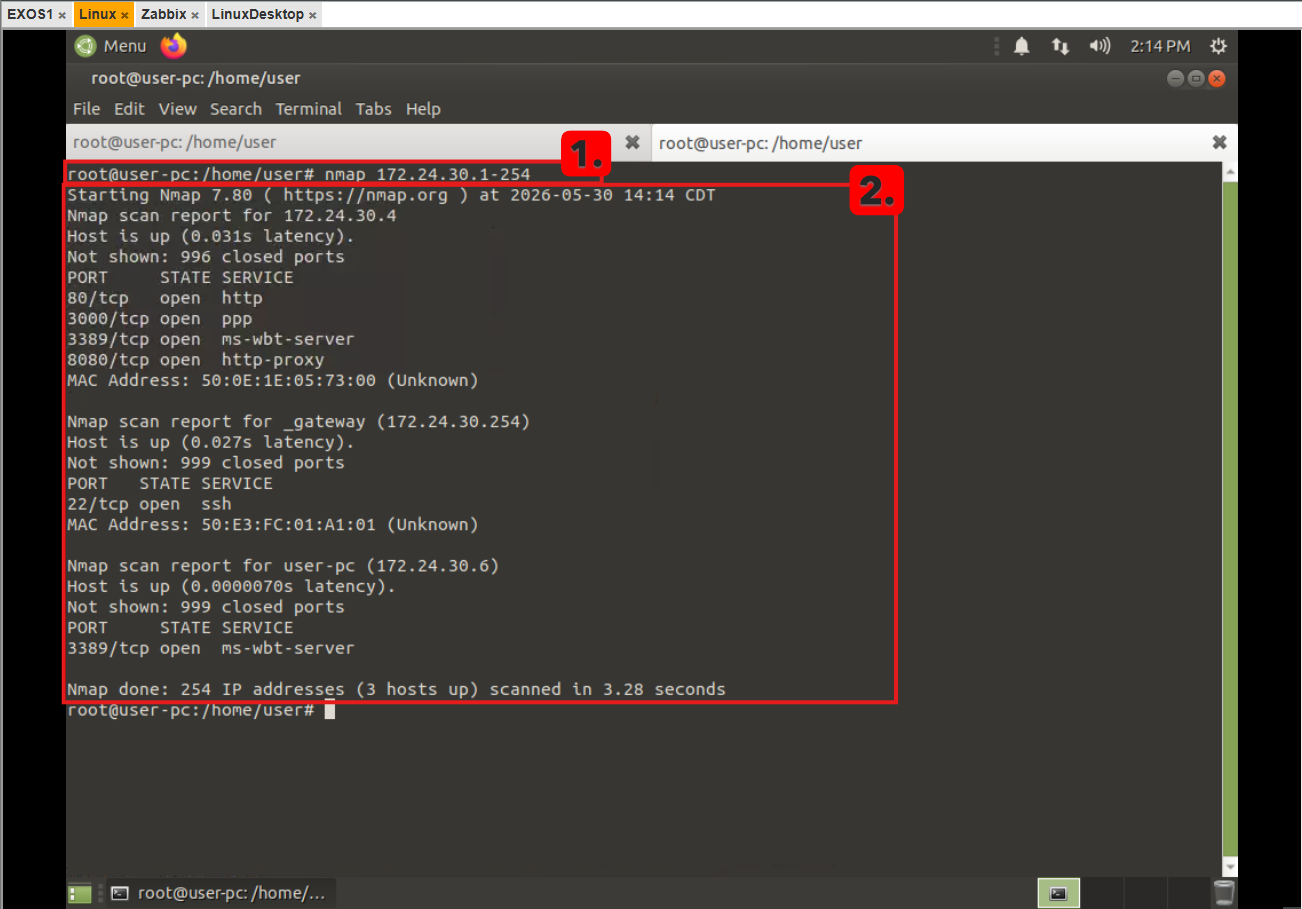
\includegraphics[width=1\linewidth]{fig/nmap3.png}
    \caption{Varredura de portas utilizando o Nmap; 1. Comando para realizar a varredura de portas em um intervalo de endereços IP; 
    2. Resultado da varredura indicando os endereços IP disponíveis na rede, as portas abertas e os serviços correspondentes}
    \label{fig:nmap3}
\end{figure}


Já na Figura \ref{fig:nmap4}, foi utilizado o comando \textit{nmap 172.24.30.254 -sS}, 
que realiza uma varredura de portas utilizando o método de varredura TCP SYN,
 o resultado da varredura indicou que a porta 22 (SSH) estava aberta no gateway e mostrou o MAC Address.

\begin{figure}[H]
    \centering
    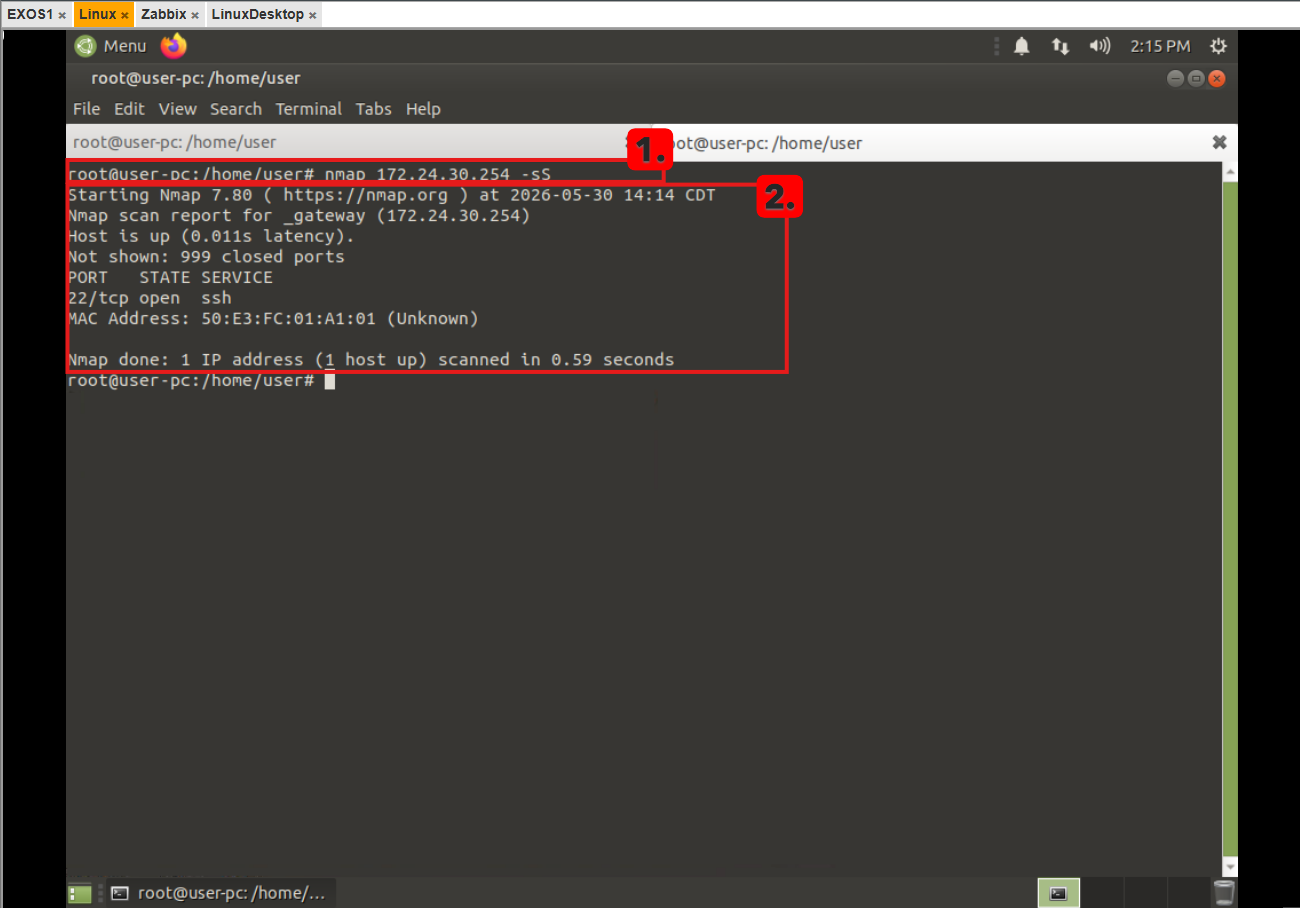
\includegraphics[width=1\linewidth]{fig/nmap4.png}
    \caption{Varredura de portas utilizando o Nmap; 
    1. Comando para realizar a varredura de portas utilizando o método de varredura TCP SYN; 
    2. Resultado da varredura indicando as portas abertas e os serviços correspondentes}
    \label{fig:nmap4}
\end{figure}

Em seguida, por meio do comando \textit{nmap 172.24.30.1-254 -sV}, mostrado na Figura \ref{fig:nmap5},\ref{fig:nmap6} e \ref{fig:nmap7}, 
foi realizada uma varredura de portas e identificação do tipo de serviços utilizando o método de varredura 
TCP SYN em um intervalo de endereços IP, o resultado da varredura indicou quais IPs estavam disponíveis 
na rede, quais portas estavam abertas em cada um dos hosts, 
bem como os serviços e a versão dos serviços correspondentes a essas portas.


\begin{figure}[H]
    \centering
    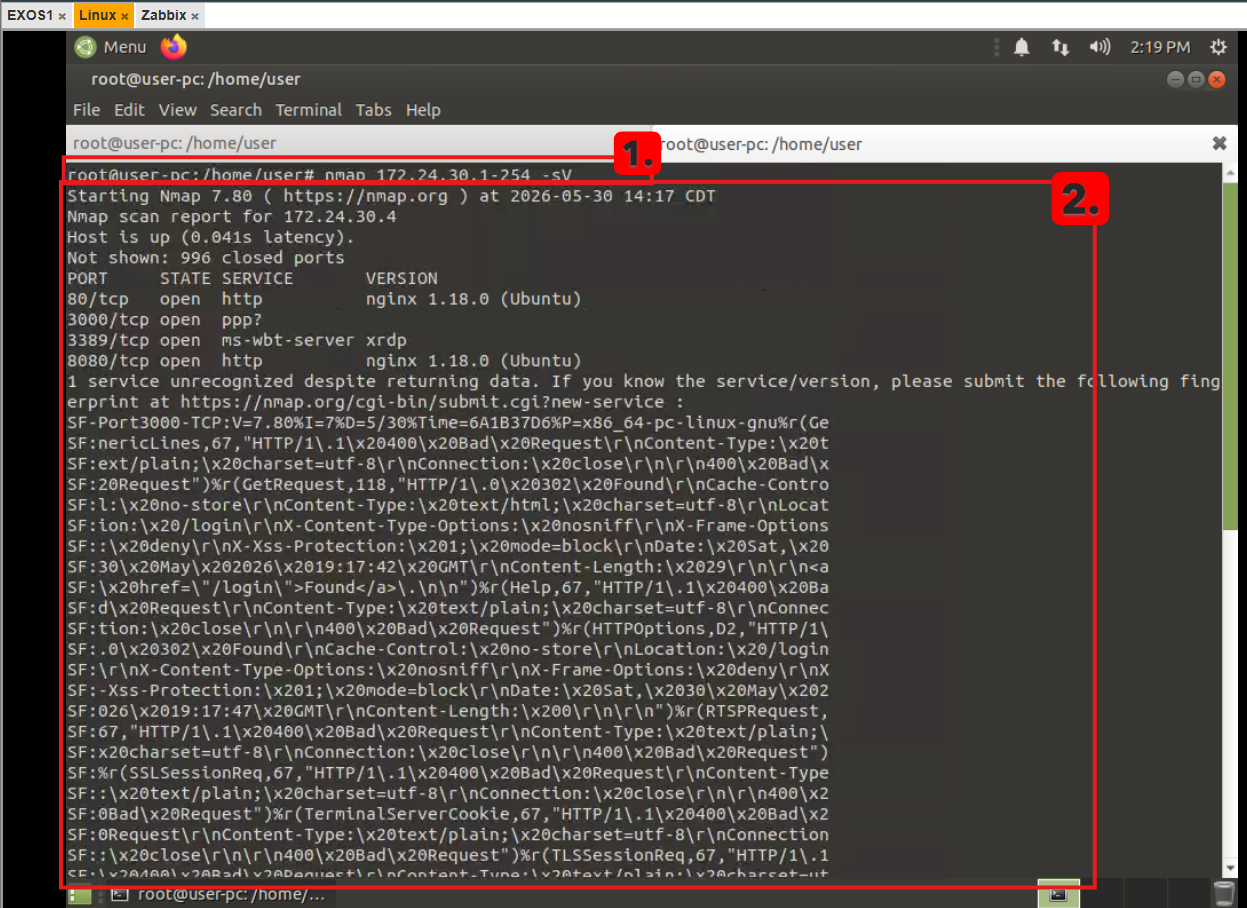
\includegraphics[width=1\linewidth]{fig/nmap5.png}
    \caption{Varredura de portas utilizando o Nmap 1; 
     1. Comando para realizar a varredura de portas e identificação do tipo de serviços;
     2. Resultado da varredura indicando os endereços IP disponíveis na rede }
    \label{fig:nmap5}
\end{figure}


\begin{figure}[H]
    \centering
    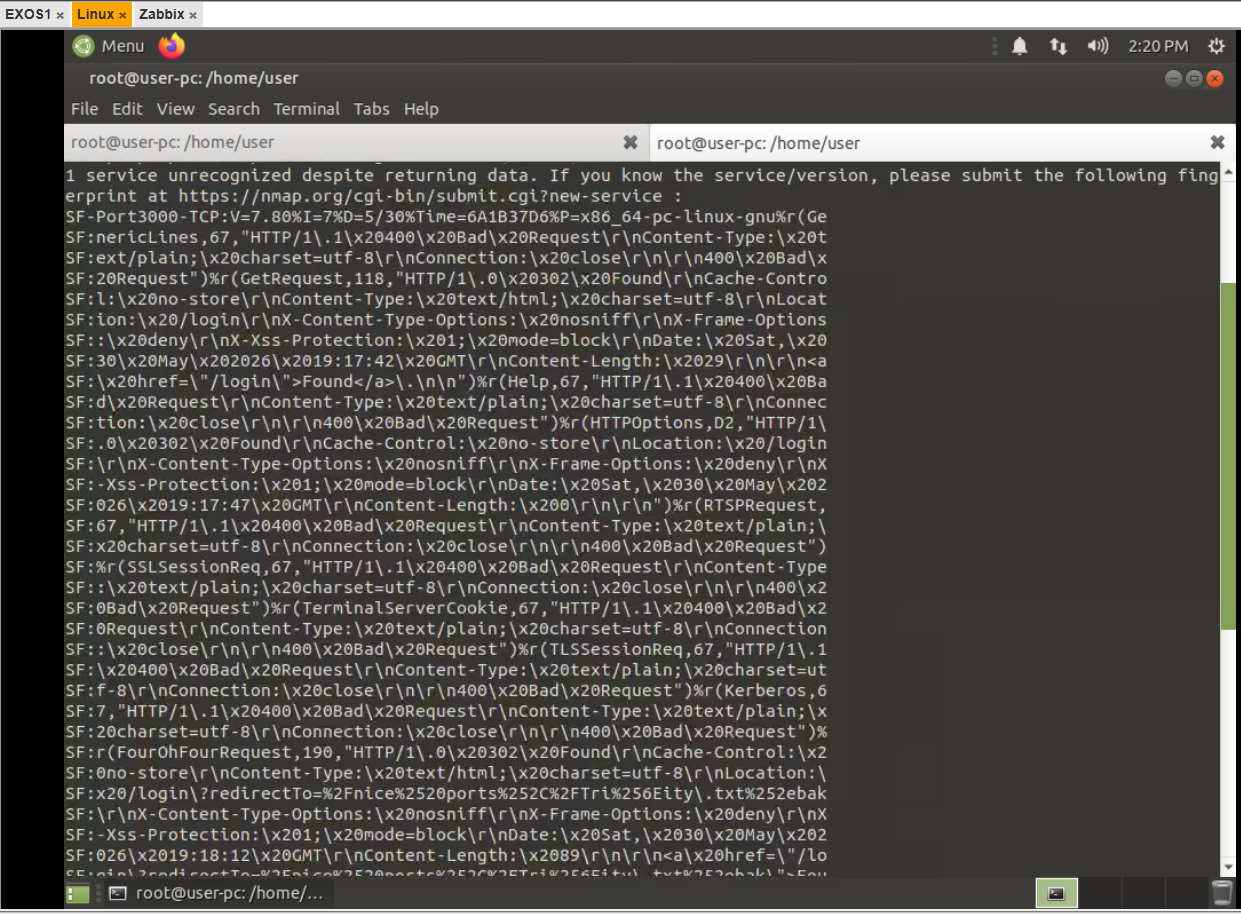
\includegraphics[width=1\linewidth]{fig/nmap6.png}
    \caption{Resultado da varredura utilizando o Nmap 2}
    \label{fig:nmap6}
\end{figure}

\begin{figure}[H]
    \centering
    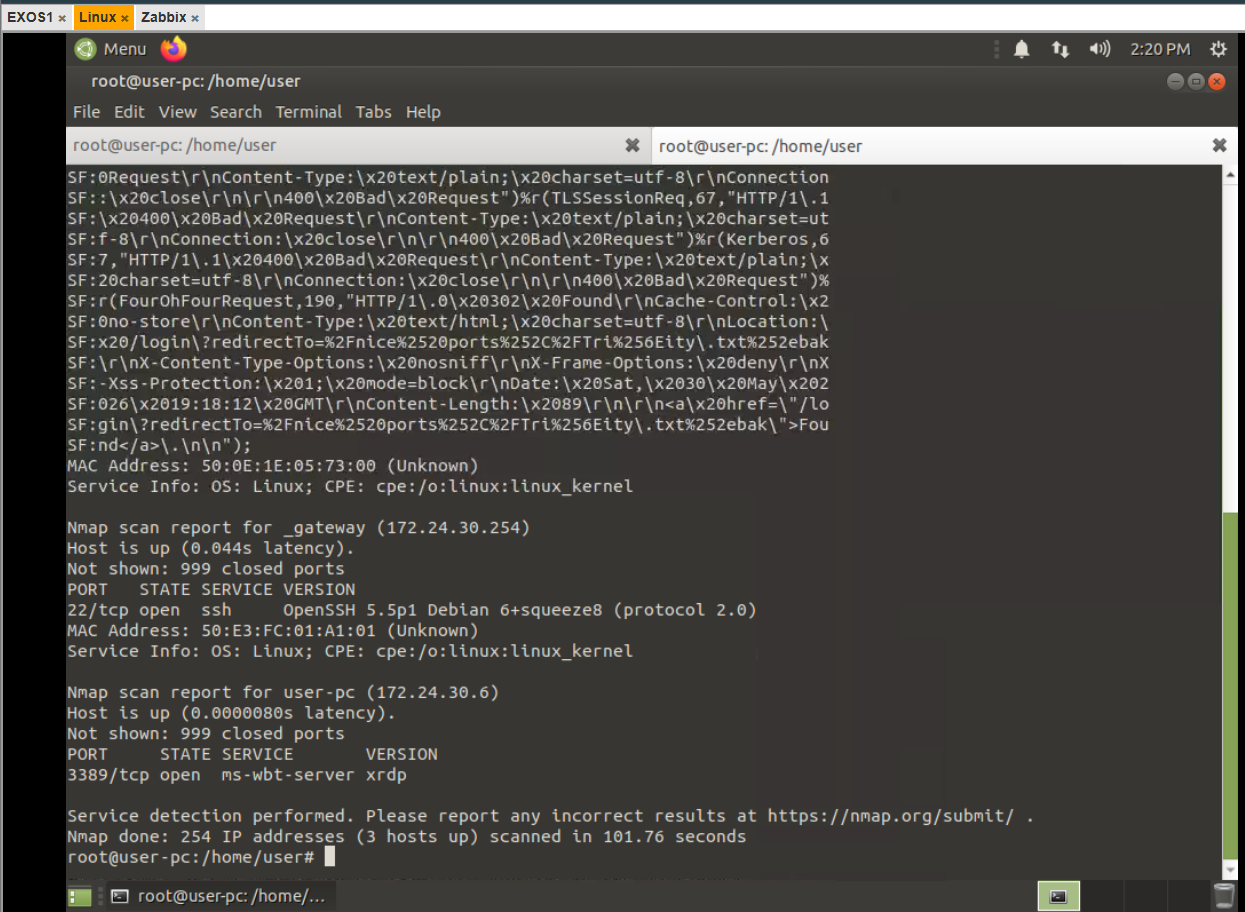
\includegraphics[width=1\linewidth]{fig/nmap7.png}
    \caption{Resultado da varredura utilizando o Nmap 3}
    \label{fig:nmap7}
\end{figure}

Como última simulação, foi utilizado o comando \textit{nmap 172.24.30.254 -A}. Por meio desse comando, é possível 
detectar o SO, a versão, verificar scripts e traceroute. Como resultado da varredura, 
foi possível identificar o sistema operacional do gateway, a versão do serviço SSH,
 bem como a presença de scripts de segurança e o caminho de rede para o host alvo.

\begin{figure}[H]
    \centering
    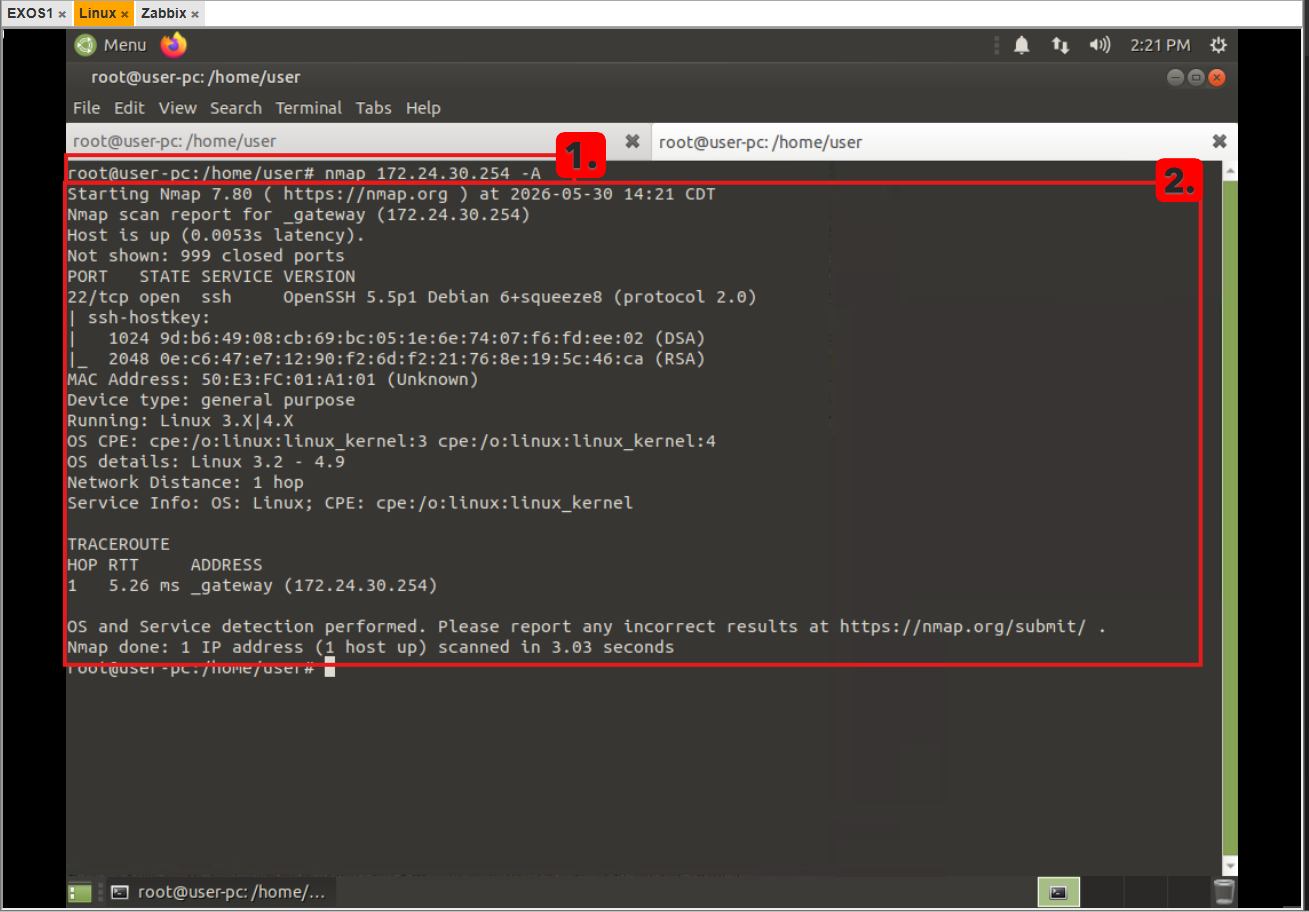
\includegraphics[width=1\linewidth]{fig/nmap8.png}
    \caption{Resultado da varredura utilizando o Nmap com a opção -A; 
    1. Comando para realizar a varredura de portas e identificação do tipo de serviços utilizando a opção -A; 
    2. Resultado da varredura indicando o sistema operacional, a versão do serviço SSH}
    \label{fig:nmap8}
\end{figure}

\subsection{UFW}


Para a primeira simulação, foi utilizado o comando \textit{ufw allow ssh}, 
mostrado na Figura \ref{fig:ufw1}, 
para permitir conexões SSH utilizando o UFW.
 O resultado do comando indicou que a regra foi adicionada com sucesso. Em seguida, foi utilizado
  o comando \textit{ufw status} para verificar o status do UFW,
  confirmando que a regra de permissão para conexões SSH estava ativa.
\begin{figure}[H]
    \centering
    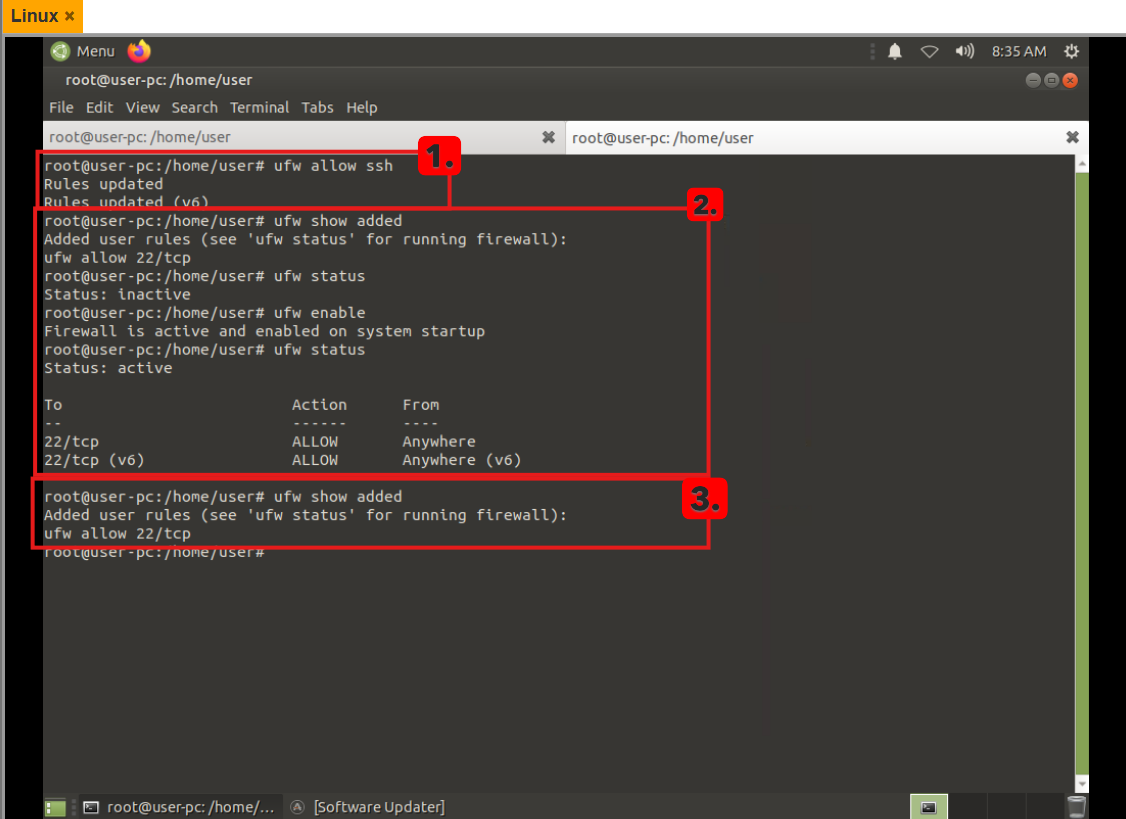
\includegraphics[width=1\linewidth]{fig/ufw1.png}
    \caption{Permitindo conexões SSH utilizando o UFW; 
    1. Comando para permitir conexões SSH; 
    2. Resultado do comando indicando que a regra foi adicionada com sucesso; 
    3. Comando para verificar o status do UFW;}
    \label{fig:ufw1}
\end{figure}

Na Figura \ref{fig:ufw2}, 
é possível observar o resultado do teste de conexão SSH entre o 
Host Linux e o Roteador ROT-ACME,
 indicando que a conexão foi estabelecida com sucesso, confirmando que a regra de permissão para
  conexões SSH estava funcionando corretamente.

\begin{figure}[H]
    \centering
    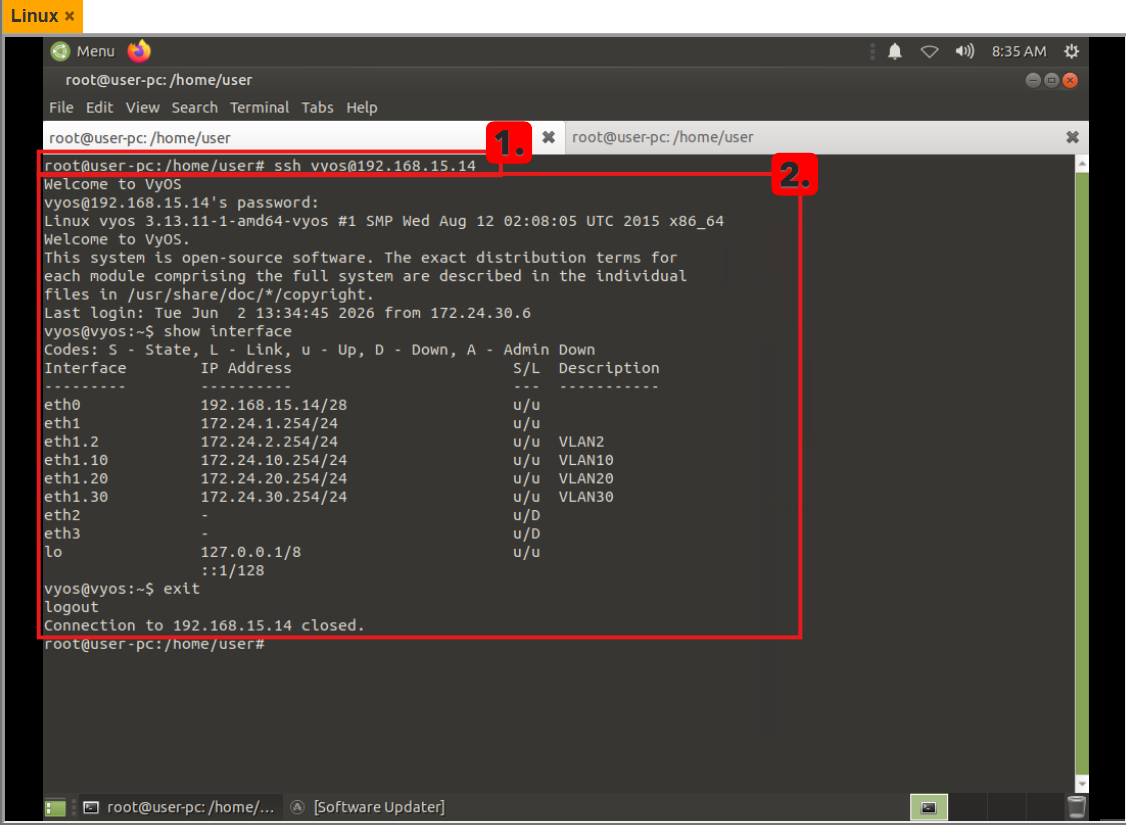
\includegraphics[width=1\linewidth]{fig/ufw2.png}
    \caption{Conexão SSH permitida utilizando o UFW; 
    1. Comando para realizar o SSH para o Roteador ROT-ACME;
    2. Resultado do comando indicando que a conexão SSH foi estabelecida com sucesso}
    \label{fig:ufw2}
\end{figure}

Em seguida, por meio do comando \textit{ufw deny ssh}, 
mostrado na Figura \ref{fig:ufw3},
 foi possível desabilitar o SSH utilizando o UFW. O resultado do comando 
 indicou que a regra de bloqueio para conexões SSH foi adicionada com sucesso. 
 Em seguida, foi utilizado o comando \textit{ufw status} para verificar o status do UFW, 
 confirmando que a regra de bloqueio para conexões SSH estava ativa.

\begin{figure}[H]
    \centering
    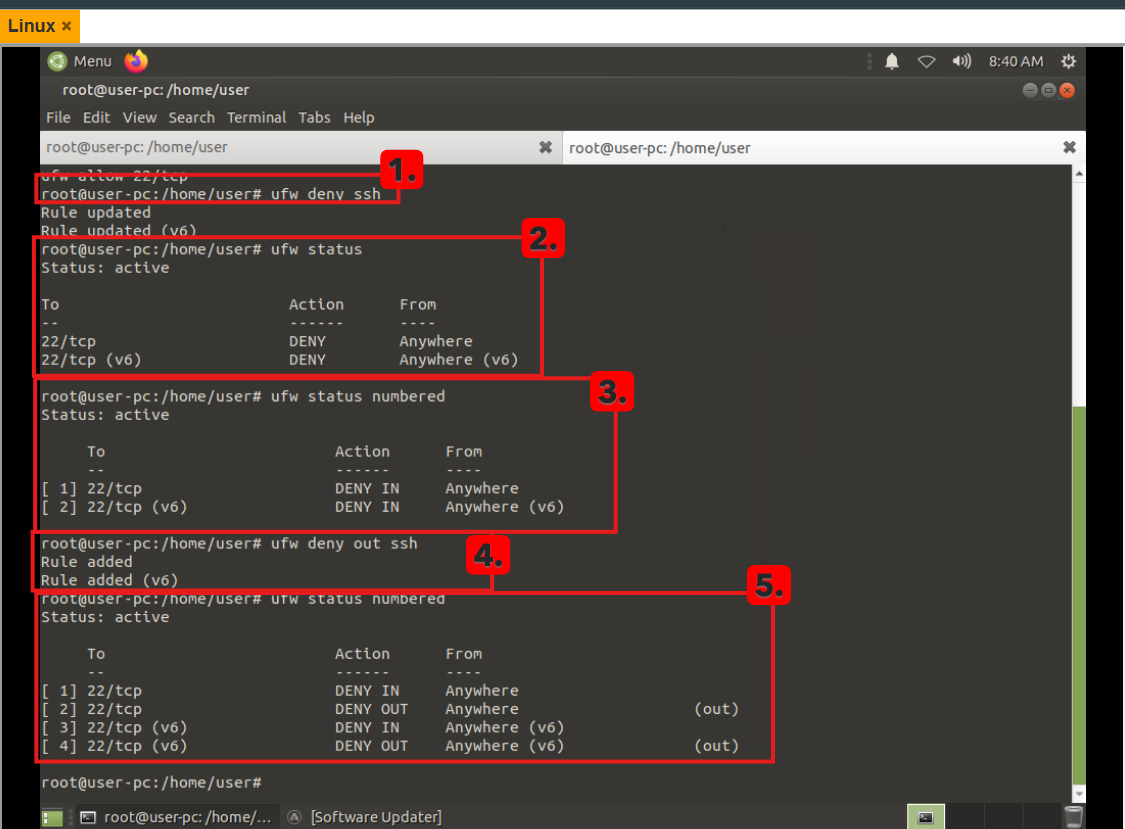
\includegraphics[width=1\linewidth]{fig/ufw3.png}
    \caption{Desabilitando o SSH utilizando o UFW;
     1. Comando para desabilitar o SSH para o Host Linux; 
     2. Resultado do comando indicando que a regra foi adicionada com sucesso;
     3. Comando para verificar o status do UFW enumerando as regras ativas;
     4. Comando para desabilitar o SSH do Host Linux para outros hosts utilizando o UFW;
     5. Resultado do comando indicando que a regra foi adicionada com sucesso;}
    \label{fig:ufw3}
\end{figure}

A Figura \ref{fig:ufw4} mostra o resultado do teste de
conexão SSH entre o Host Linux e o Roteador ROT-ACME, indicando que a conexão foi bloqueada 
com sucesso, confirmando que a regra de bloqueio para conexões SSH estava funcionando corretamente.

\begin{figure}[H]
    \centering
    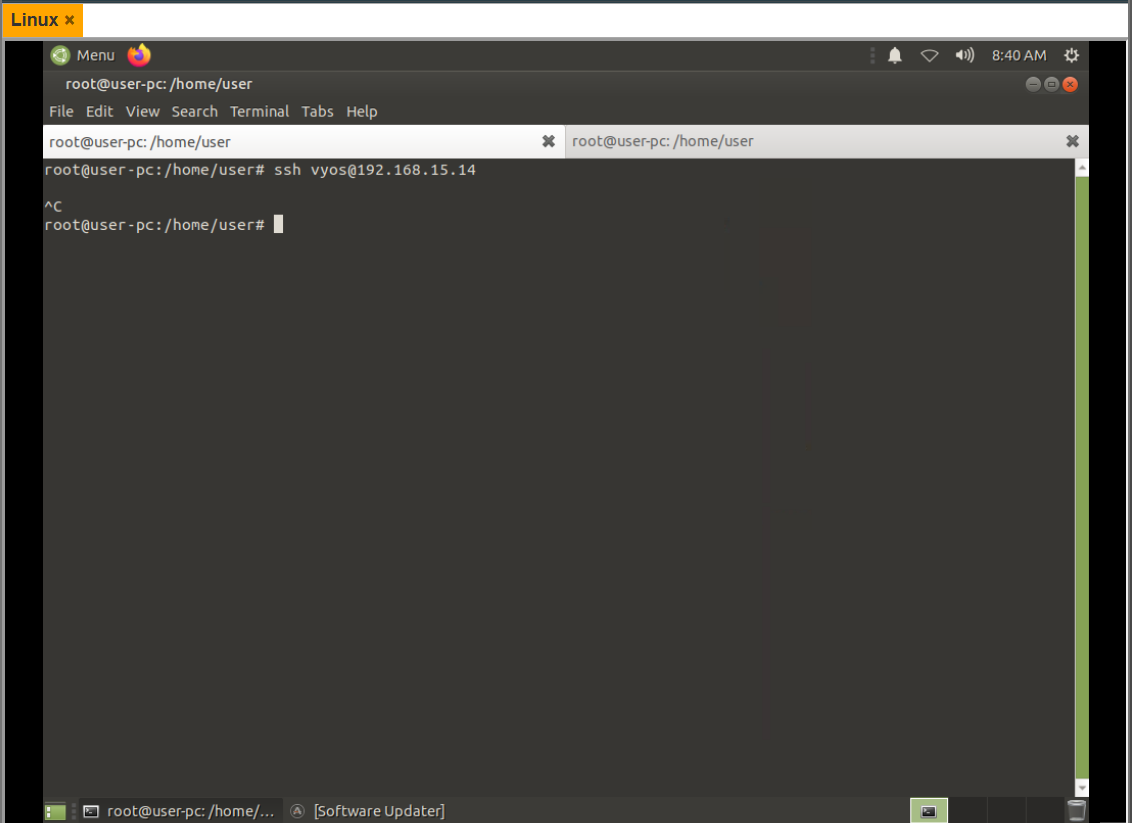
\includegraphics[width=1\linewidth]{fig/ufw4.png}
    \caption{Resultado do bloqueio do SSH utilizando o UFW;}
    \label{fig:ufw4}
\end{figure}

Na terceira simulação, foi utilizado o comando 
\textit{ufw delete deny ssh}, mostrado na Figura \ref{fig:ufw5}, para deletar a regra de 
bloqueio do SSH utilizando o UFW. O resultado do comando indicou que a regra foi deletada 
com sucesso. Em seguida, foi utilizado o comando \textit{ufw status}.       

\begin{figure}[H]
    \centering
    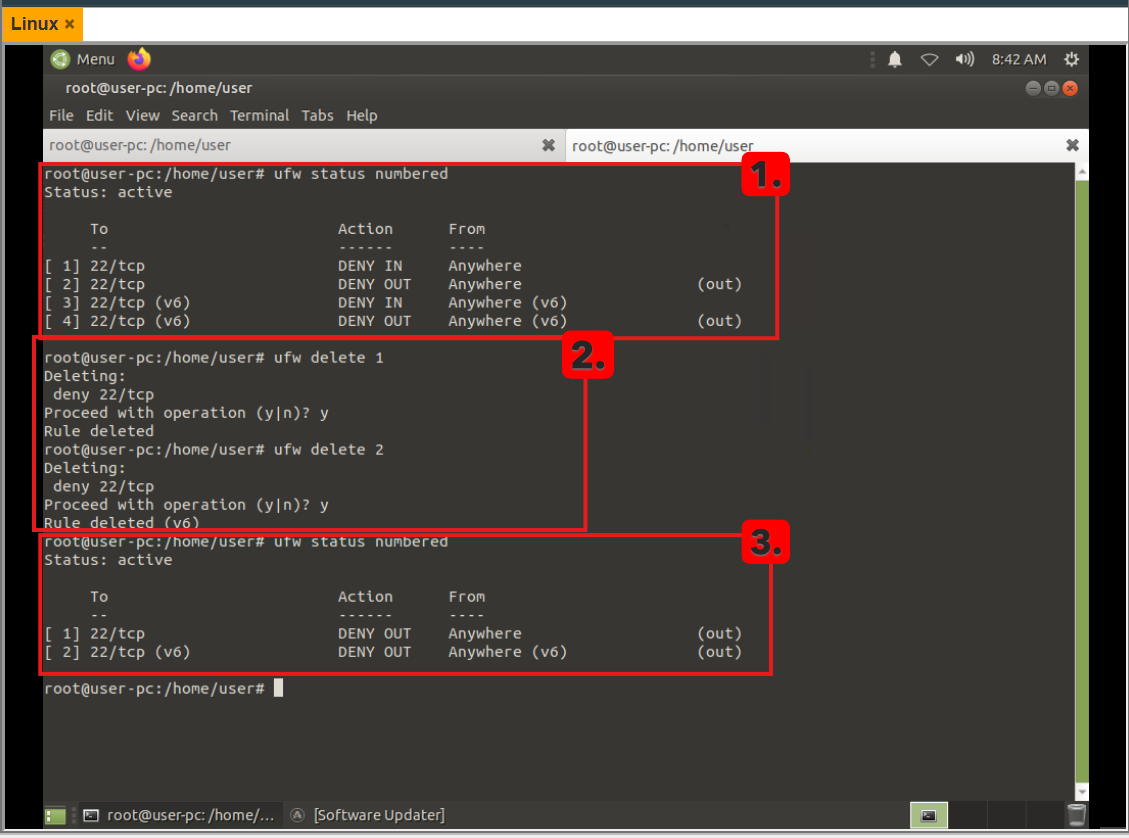
\includegraphics[width=1\linewidth]{fig/ufw5.png}
    \caption{Exclusão de uma regra no UFW;
    1. Comando para mostrar as regras ativas do UFW enumerando as regras;
    2. Comando para deletar a regra de bloqueio do SSH utilizando o número da regra;
    3. Resultado do comando indicando que a regra foi deletada com sucesso;}
    \label{fig:ufw5}
\end{figure}

Para visualizar a lista de serviços ativos, 
foi utilizado o comando \textit{ufw status}, mostrado na Figura \ref{fig:ufw6}.
 O resultado do comando indicou que a regra de permissão para conexões SSH estava ativa. 
 Em seguida, foi utilizado o comando \textit{ufw disable} para desabilitar o UFW,
  e o resultado do comando indicou que o firewall foi desabilitado com sucesso.

\begin{figure}[H]
    \centering
    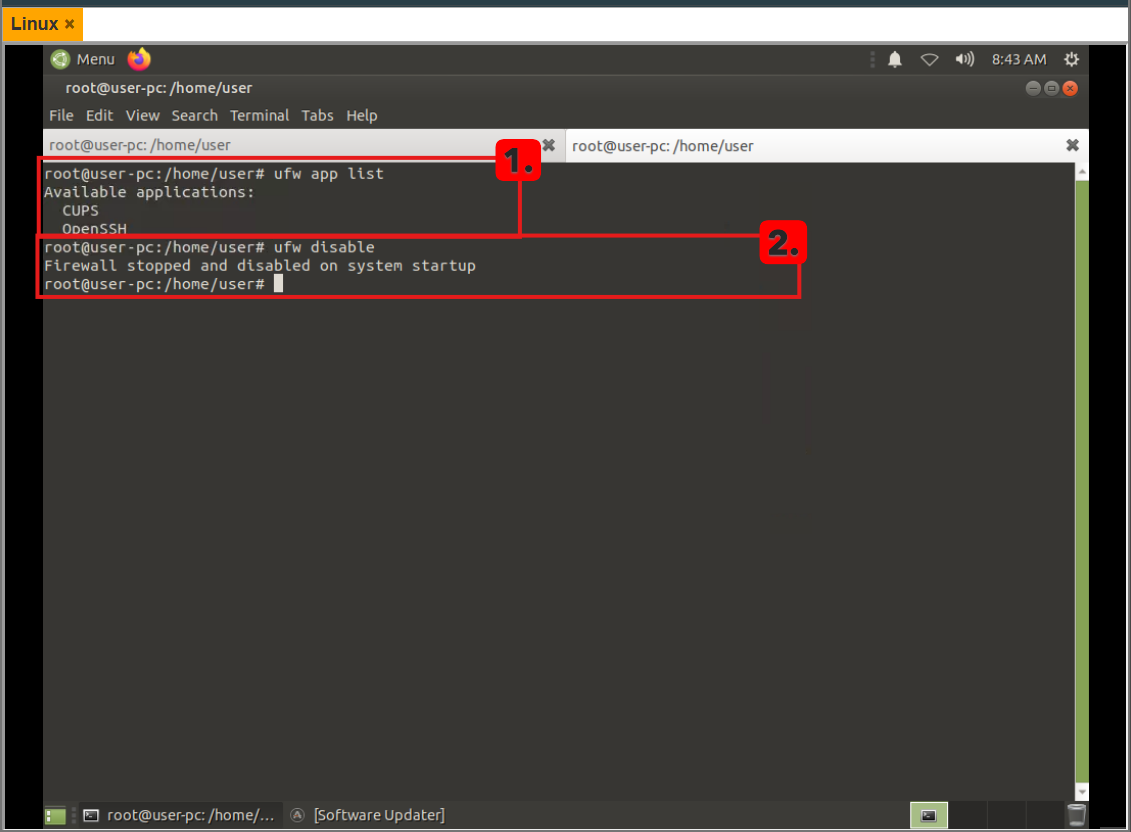
\includegraphics[width=1\linewidth]{fig/ufw6.png}
    \caption{1. Comando para visualizar a lista de serviços ativos;
    2. Comando para desabilitar o UFW;}
    \label{fig:ufw6}
\end{figure}

Já na última simulação, foi utilizado o comando \textit{ufw default enable deny incoming}, mostrado na 
Figura \ref{fig:ufw7}, para configurar a política padrão do UFW para negar conexões de entrada. 
O resultado do comando indicou que a política padrão para conexões de entrada foi 
configurada com sucesso. Em seguida, foi utilizado o comando \textit{ufw default allow outgoing} 
para configurar a política padrão do UFW para permitir conexões de saída,
 e o resultado do comando indicou que a política padrão para conexões de saída foi configurada com sucesso.

\begin{figure}[H]
    \centering
    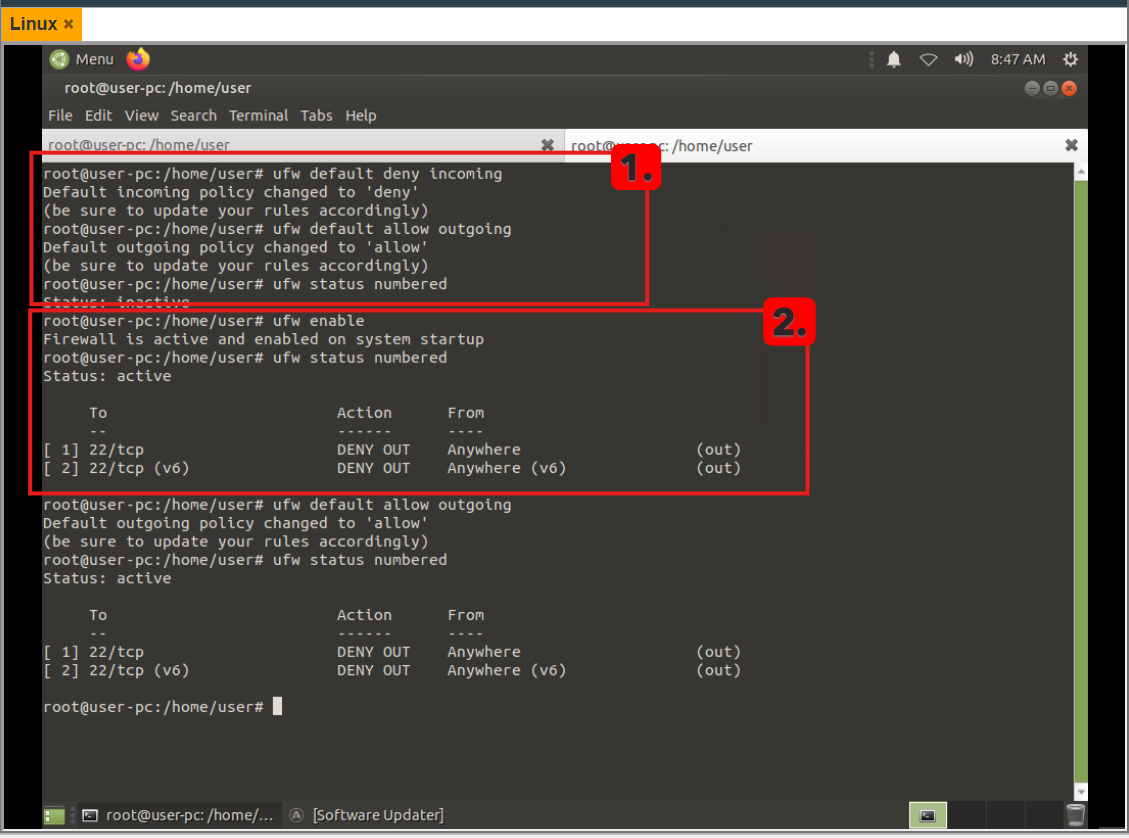
\includegraphics[width=1\linewidth]{fig/ufw7.png}
    \caption{1. Comando para bloquear política de entrada; 
    2. Comando para permitir política de saída;}
    \label{fig:ufw7}
\end{figure}

\subsection{SNORT}

Para as simulações com o Snort, inicialmente foi testado o envio de notificações no ambiente Linux
utilizando o comando \textit{notify-send}, como mostrado na Figura \ref{fig:snort1}. Esse teste foi
realizado para verificar se o sistema conseguia exibir alertas na interface gráfica, recurso utilizado
posteriormente para apresentar as notificações geradas a partir das detecções do Snort.

\begin{figure}[H]
    \centering
    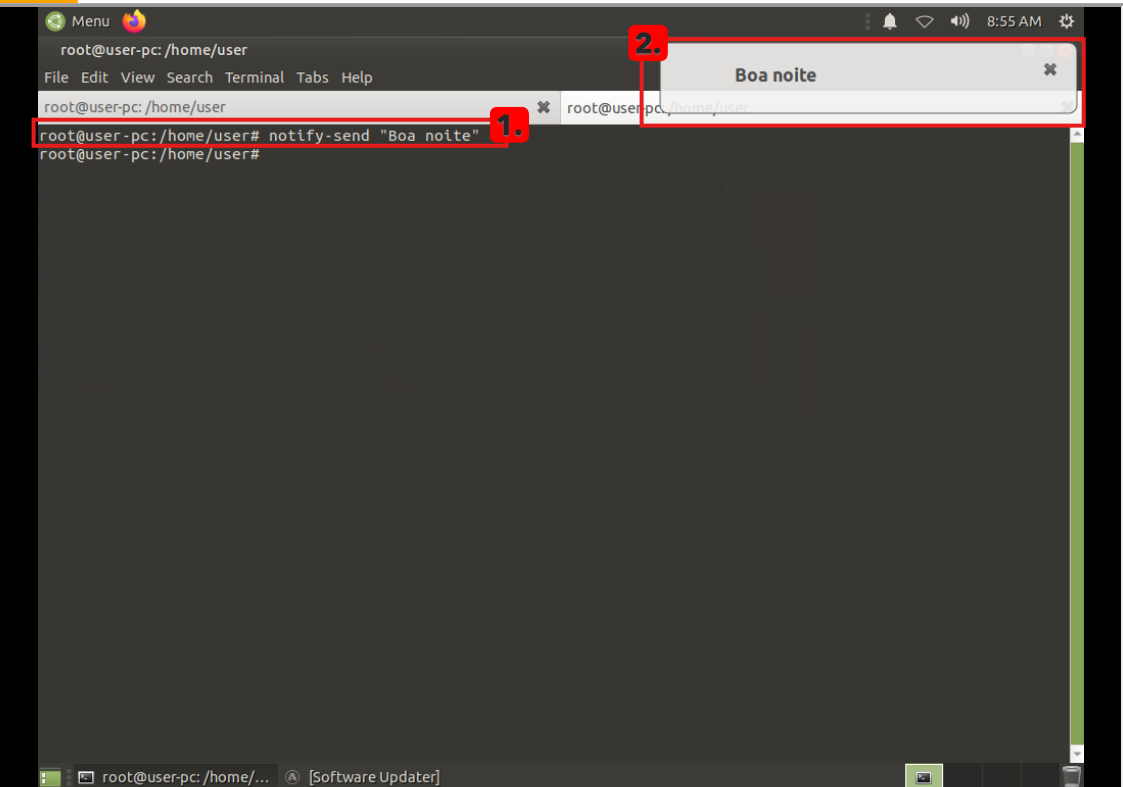
\includegraphics[width=1\linewidth]{fig/snort1.png}
    \caption{Notificação utilizando o notify-send;
     1. Comando notify-send para enviar uma notificação; 
     2. Resultado do comando indicando que a notificação foi enviada com sucesso}
    \label{fig:snort1}
\end{figure}


Em seguida, foi adicionada uma regra personalizada no arquivo \textit{/etc/snort/rules/local.rules},
conforme apresentado na Figura \ref{fig:snort2}. A regra configurada utiliza a ação \textit{alert}
para pacotes do tipo ICMP, permitindo que o Snort gere um alerta sempre que for identificado tráfego
de ping na rede. A mensagem definida para o alerta foi \textit{ECMP ECHO Request detectado}, com o
identificador \textit{sid: 1000001}.

\begin{figure}[H]
    \centering
    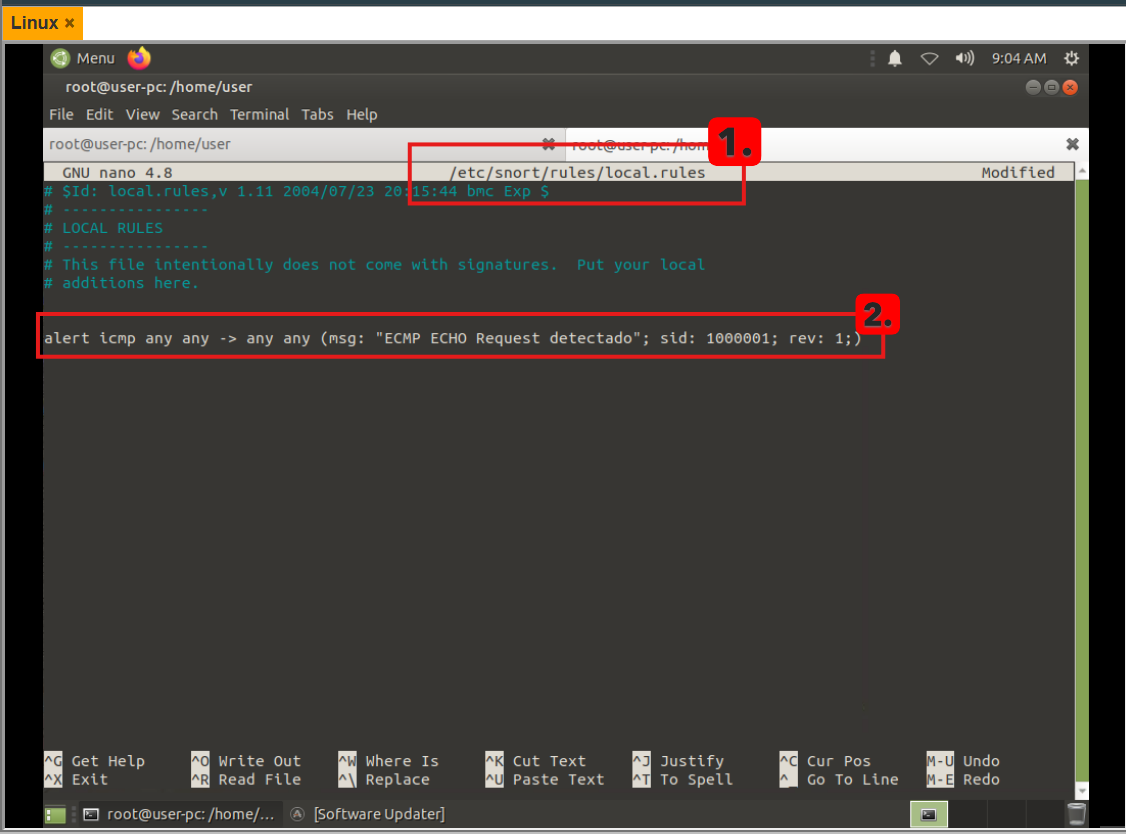
\includegraphics[width=1\linewidth]{fig/snort2.png}
    \caption{Adicionando uma regra personalizada no Snort;
     1. Caminho do arquivo de regras do Snort; 
     2. Regra personalizada para detectar tráfego ICMP;}
    \label{fig:snort2}
\end{figure}

Após a criação da regra, foi realizado um teste de conectividade com o comando \textit{ping 172.24.30.6},
partindo do LinuxDesktop para o Host Linux, como mostrado na Figura \ref{fig:snort4}. O teste gerou
pacotes ICMP Echo Request e Echo Reply, que serviram como tráfego de entrada para validar a regra
personalizada configurada no Snort.

\begin{figure}[H]
    \centering
    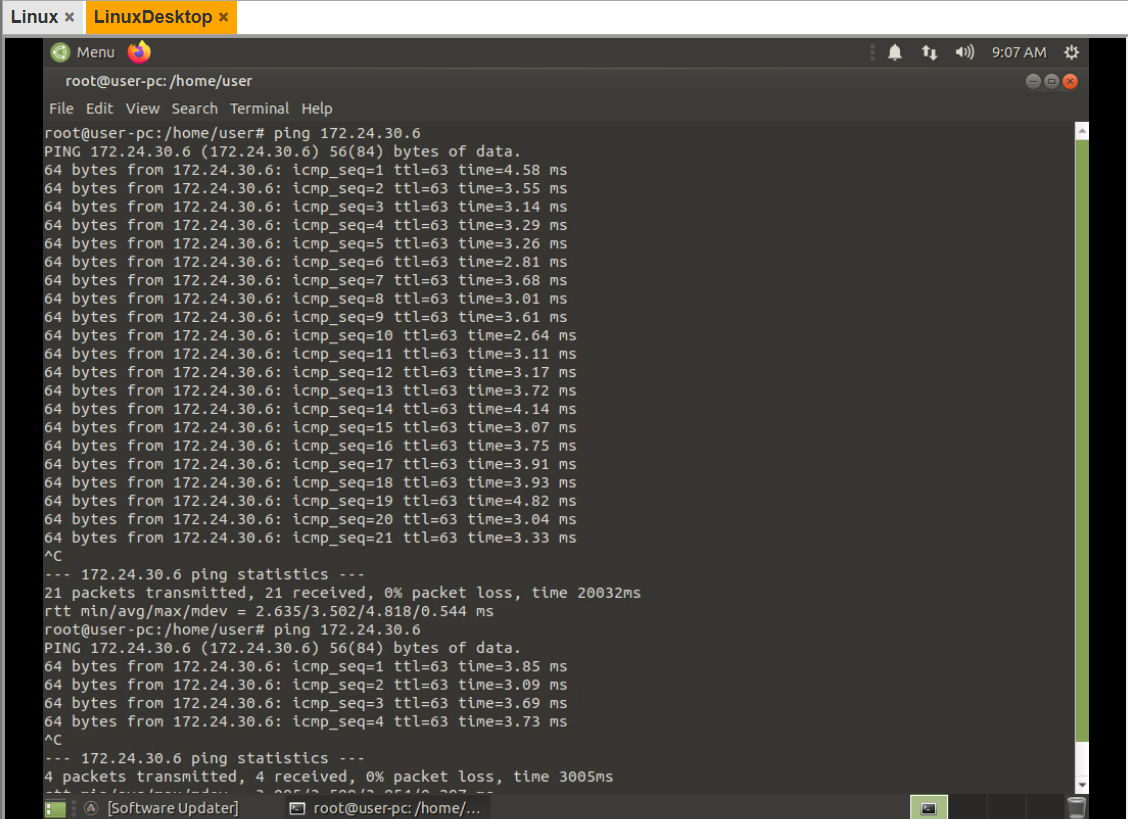
\includegraphics[width=1\linewidth]{fig/snort4.png}
    \caption{Ping realizado do LinuxDesktop para o Host Linux}
    \label{fig:snort4}
\end{figure}


Na Figura \ref{fig:snort3}, é possível observar a execução do Snort em modo console, utilizando o
arquivo de regras personalizado e a interface de rede \textit{ens3}. O comando
\textit{snort -A console -q -c /etc/snort/rules/local.rules -dev -i ens3} monitora os pacotes
capturados e exibe os alertas diretamente no terminal. Como resultado, o Snort identificou o tráfego
ICMP gerado pelo teste de ping e exibiu os alertas correspondentes, contendo os endereços IP de origem
e destino, o tipo ICMP e os dados do pacote.

\begin{figure}[H]
    \centering
    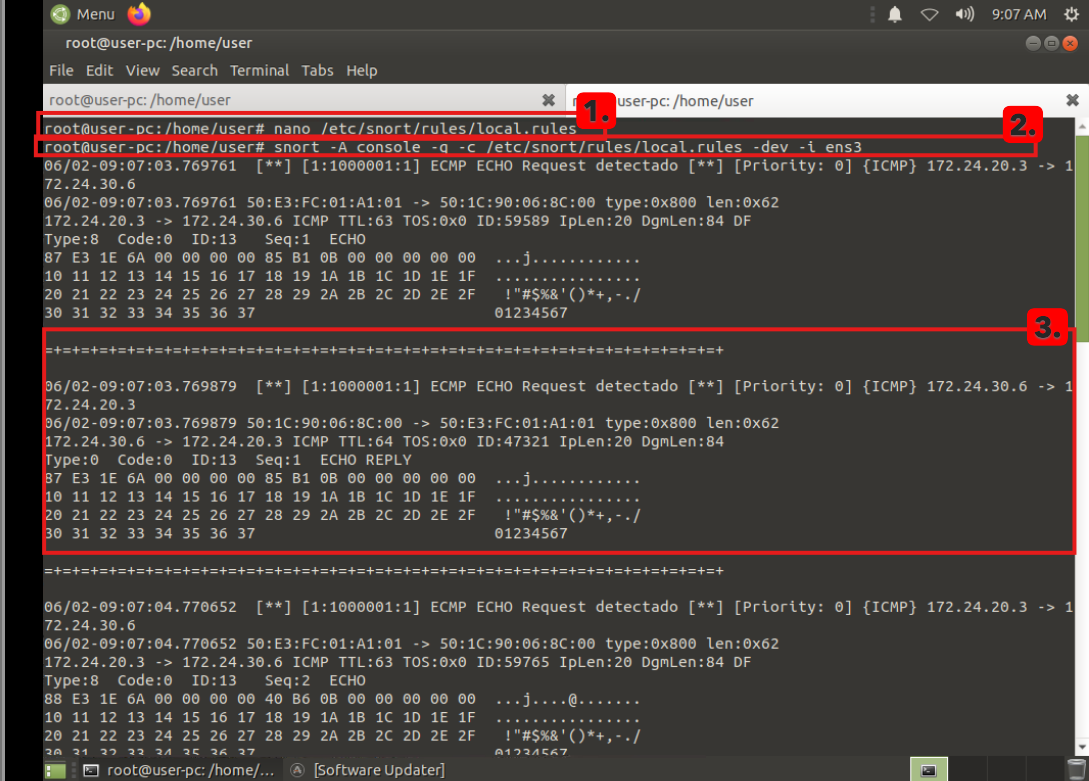
\includegraphics[width=1\linewidth]{fig/snort3.png}
    \caption{1. Comando para acessar o arquivo de regras do Snort;
    2. Execução do Snort para monitorar o tráfego de rede e detectar pacotes ICMP;
    3. Resultado do comando indicando que um pacote ICMP foi detectado
    }
    \label{fig:snort3}
\end{figure}



Na segunda simulação, o Snort foi executado novamente, porém redirecionando a saída para o arquivo
\textit{infoSnort.txt}, conforme mostrado na Figura \ref{fig:snort5}. Após a interrupção da captura,
foi utilizado o comando \textit{notify-send "\$(cat infoSnort.txt)"} para enviar o conteúdo do arquivo
como uma notificação do sistema. Dessa forma, os alertas detectados pelo Snort puderam ser visualizados
fora do terminal.

\begin{figure}[H]
    \centering
    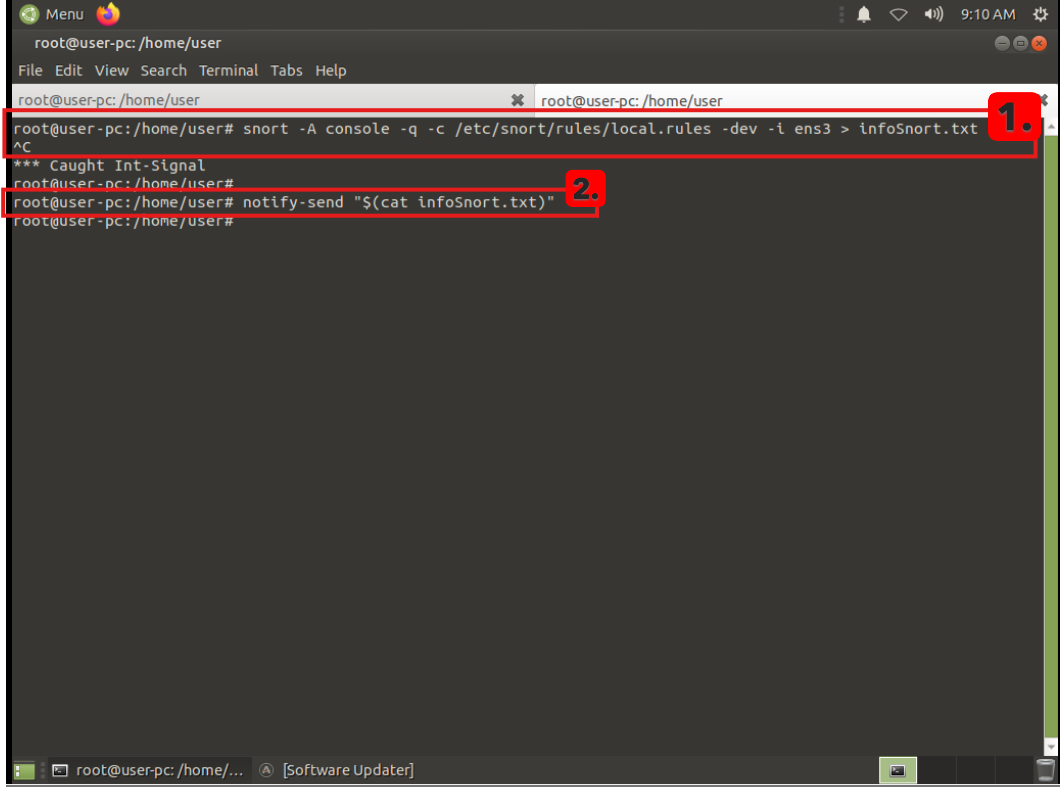
\includegraphics[width=1\linewidth]{fig/snort5.png}
    \caption{1. Comando para executar o snort no arquivo infoSnort.txt;
    2. Comando para visualizar o conteúdo do arquivo infoSnort.txt;}
    \label{fig:snort5}
\end{figure}

A Figura \ref{fig:snort6} apresenta o resultado da notificação gerada a partir do arquivo
\textit{infoSnort.txt}. Nela, é possível observar os alertas de detecção do tráfego ICMP, incluindo
requisições e respostas entre os hosts 172.24.20.3 e 172.24.30.6. Esse resultado confirma que a regra
personalizada foi acionada corretamente e que a saída do Snort pode ser reaproveitada para gerar
avisos visuais no sistema.

\begin{figure}[H]
    \centering
    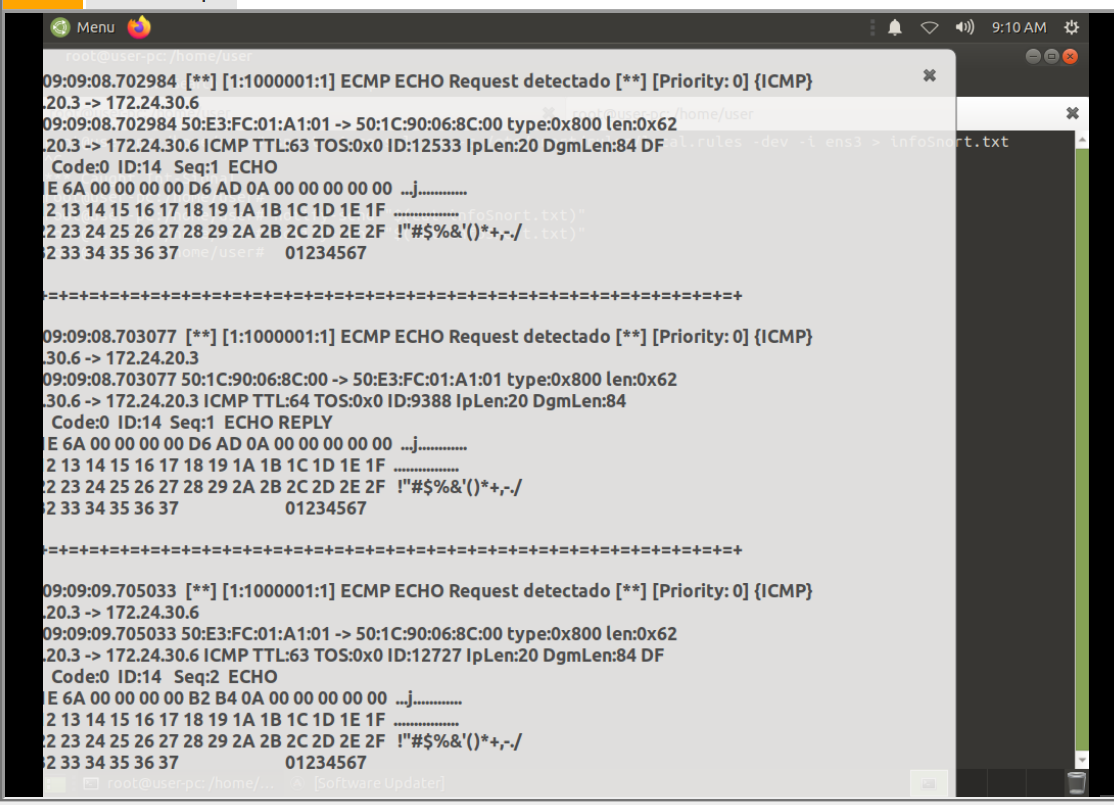
\includegraphics[width=1\linewidth]{fig/snort6.png}
    \caption{Resultado do arquivo infoSnort.txt indicando a detecção de um pacote ICMP.}
    \label{fig:snort6}
\end{figure}

Também foi configurada a saída de alertas do Snort no arquivo \textit{/etc/snort/snort.conf}, como
mostrado na Figura \ref{fig:snort7}. Nessa etapa, foi adicionada a diretiva
\textit{output alert\_fast: alert.fast}, responsável por armazenar os alertas gerados pelo Snort no
formato rápido, facilitando a leitura e o acompanhamento dos eventos detectados.

\begin{figure}[H]
    \centering
    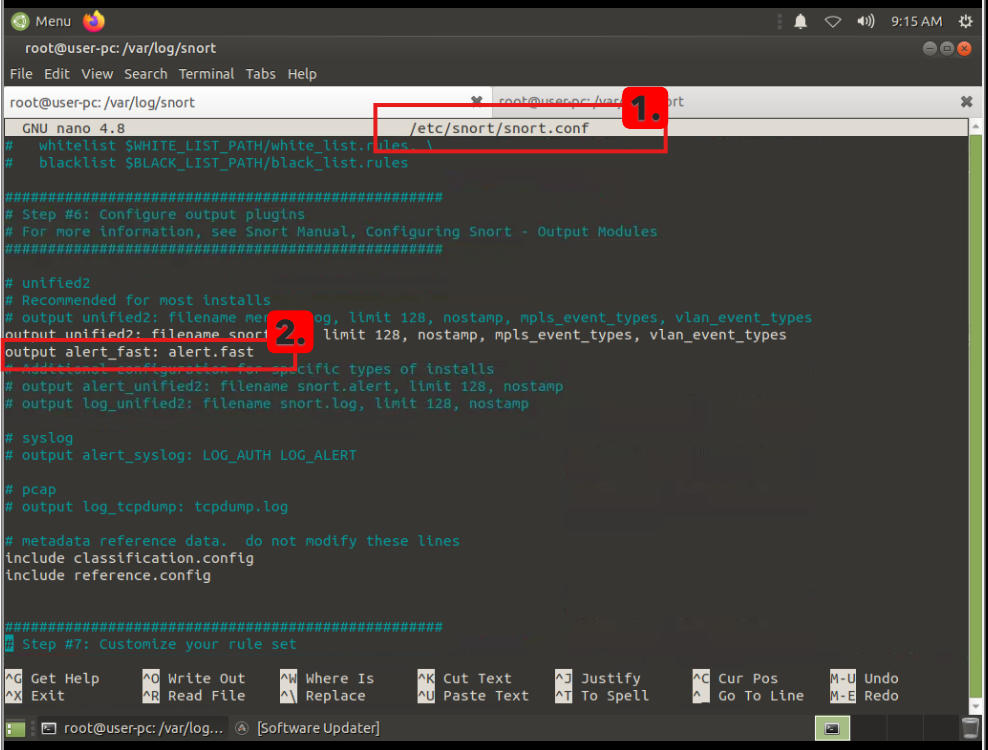
\includegraphics[width=1\linewidth]{fig/snort7.png}
    \caption{Adicionando na configuração do Snort o arquivo que será 
    utilizado para armazenar os alertas gerados pelo Snort;}
    \label{fig:snort7}
\end{figure}

Por fim, para automatizar o processo de monitoramento dos alertas do Snort, 
foram criadas regras personalizadas no arquivo \textit{/etc/snort/rules/local.rules}, como mostrado na Figura \ref{fig:snort8}. 
Essas regras foram configuradas para detectar tráfego de rede relacionado a protocolos como ICMP,
 SSH, HTTP e HTTPS. Com essas regras em vigor, o Snort será capaz de identificar e gerar alertas sempre que
  for detectado tráfego suspeito ou malicioso relacionado a esses protocolos, 
  permitindo uma resposta mais rápida e eficaz a potenciais ameaças na rede.    

\begin{figure}[H]
    \centering
    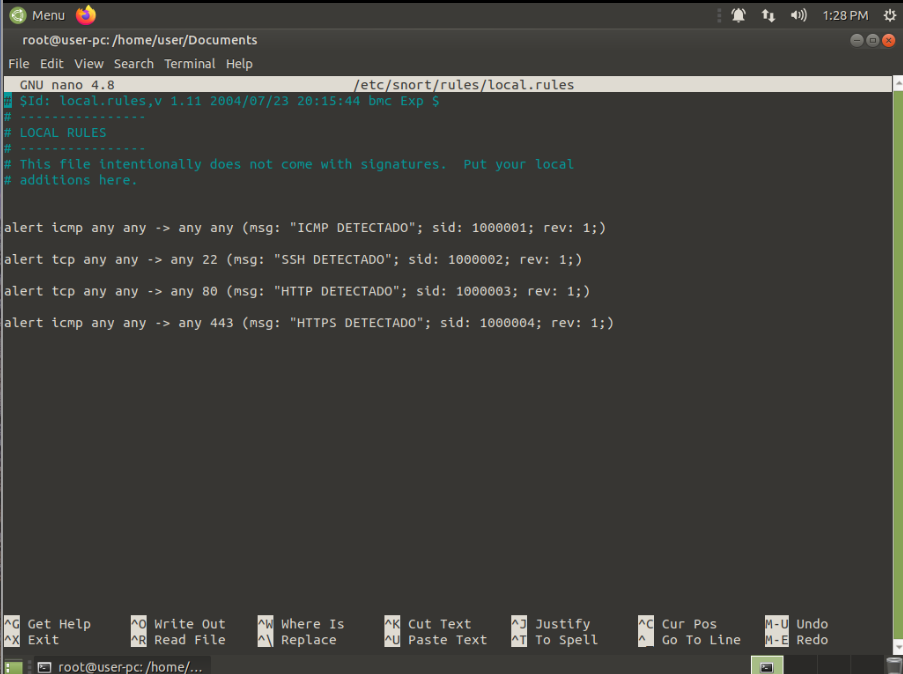
\includegraphics[width=1\linewidth]{fig/snort8.png}
    \caption{Adição de novas regras personalizadas no arquivo local.rules para detectar tráfego ICMP, SSH, HTTP e HTTPS.}
    \label{fig:snort8}
\end{figure}

Na Figura \ref{fig:snort9}, é possível observar a ativação e inicialização do serviço
\textit{snort-monitor} por meio dos comandos \textit{systemctl enable snort-monitor} e
\textit{systemctl start snort-monitor}. Em seguida, o comando \textit{systemctl status snort-monitor}
confirmou que o serviço estava ativo e em execução, indicando que o monitoramento de alertas do Snort
foi configurado corretamente.

\begin{figure}[H]
    \centering
    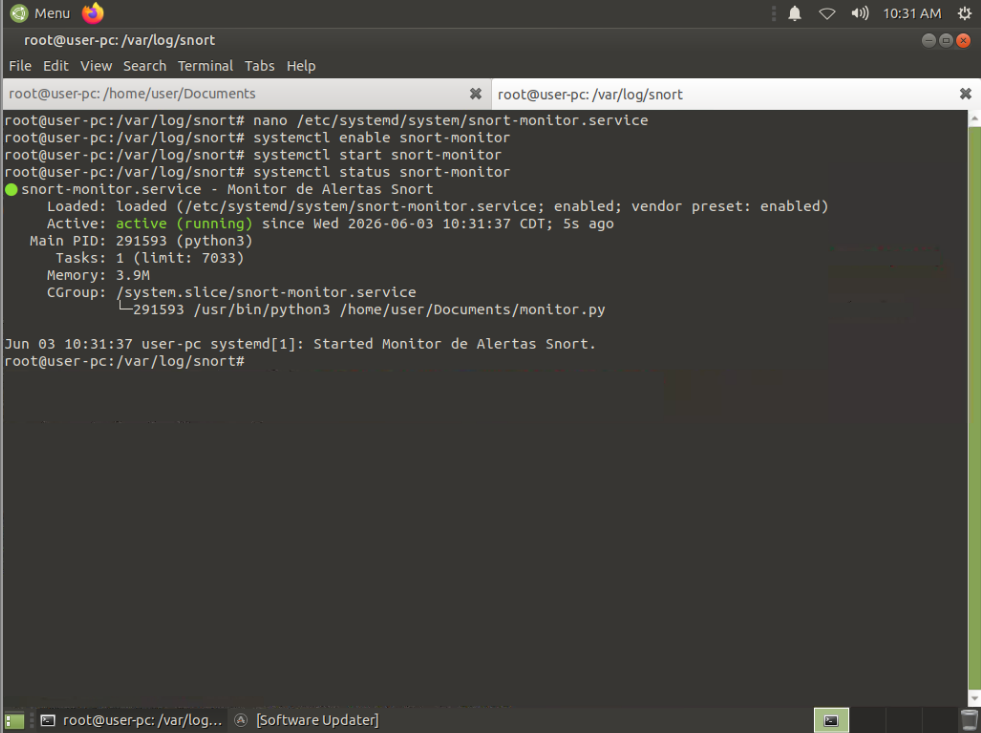
\includegraphics[width=1\linewidth]{fig/snort9.png}
    \caption{Inicialização do serviço snort-monitor;
    1. Comandos para habilitar, iniciar e verificar o status do serviço;
    2. Resultado indicando que o serviço está ativo e em execução}
    \label{fig:snort9}
\end{figure}

Foi criado o arquivo monitor.py \ref{lst:monitor} para monitorar o arquivo de alertas do Snort e 
enviar notificações utilizando o notify-send. O script lê o conteúdo do arquivo de alertas,
 verifica se há novas entradas e envia uma notificação para cada novo alerta detectado.
  O script foi configurado para ser executado periodicamente, garantindo que as notificações 
  sejam enviadas em tempo real sempre que um novo alerta for gerado pelo Snort.

Na Figura \ref{fig:snort10}, foi feita a configuração do script monitor.py para ser executado
utilizando a interface \textit{Startup Program}, que executa o arquivo monitor.py automaticamente
 durante a inicialização do sistema. Dessa forma, 
 o monitoramento dos alertas do Snort e o envio de notificações estarão ativos desde o momento em que o 
 sistema for iniciado, garantindo uma resposta imediata a qualquer evento detectado pelo Snort.

\begin{figure}[H]
    \centering
    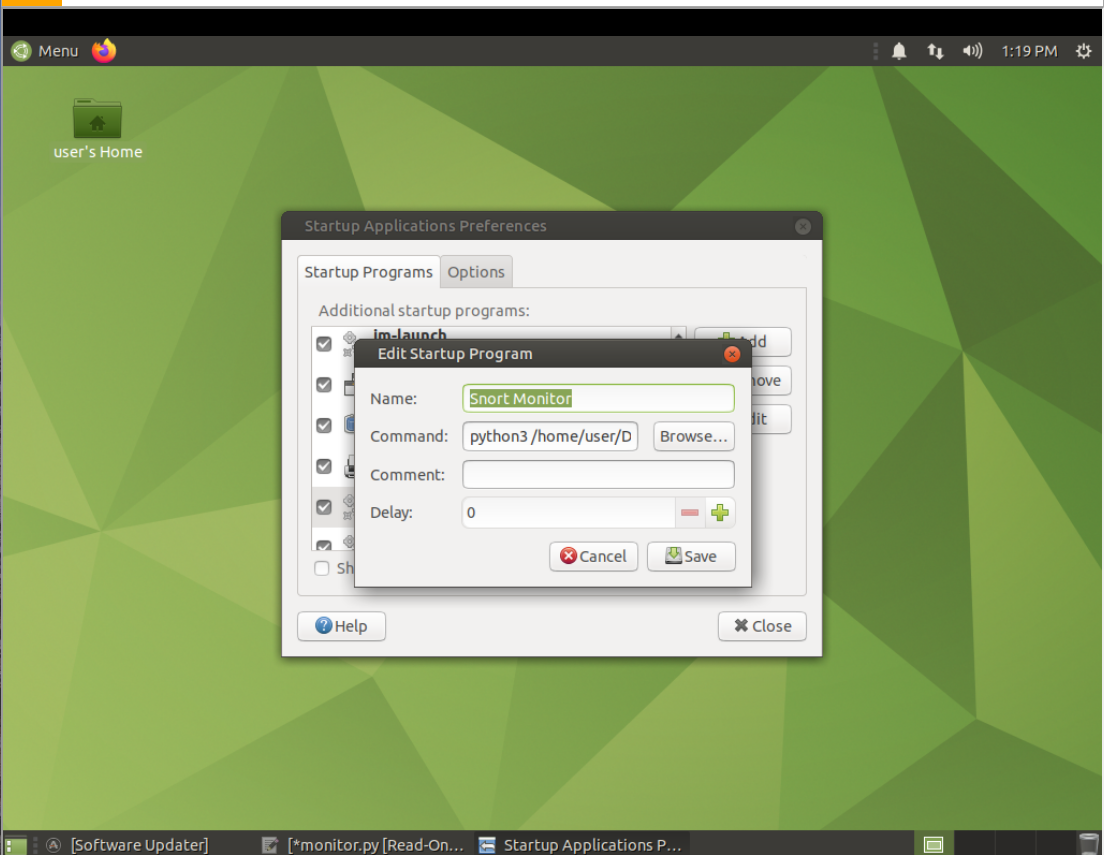
\includegraphics[width=1\linewidth]{fig/snort10.png}
    \caption{Configuração do monitor.py para inicialização automática pelo Startup Program}
    \label{fig:snort10}
\end{figure}

Já na Figura \ref{fig:snort11}, é possível observar o resultado do monitoramento do arquivo de alertas do Snort,
onde cada nova entrada no arquivo de alertas gera uma notificação utilizando o notify-send. As notificações exibem 
o conteúdo dos alertas, permitindo que o usuário seja informado em tempo real.


\begin{figure}[H]
    \centering
    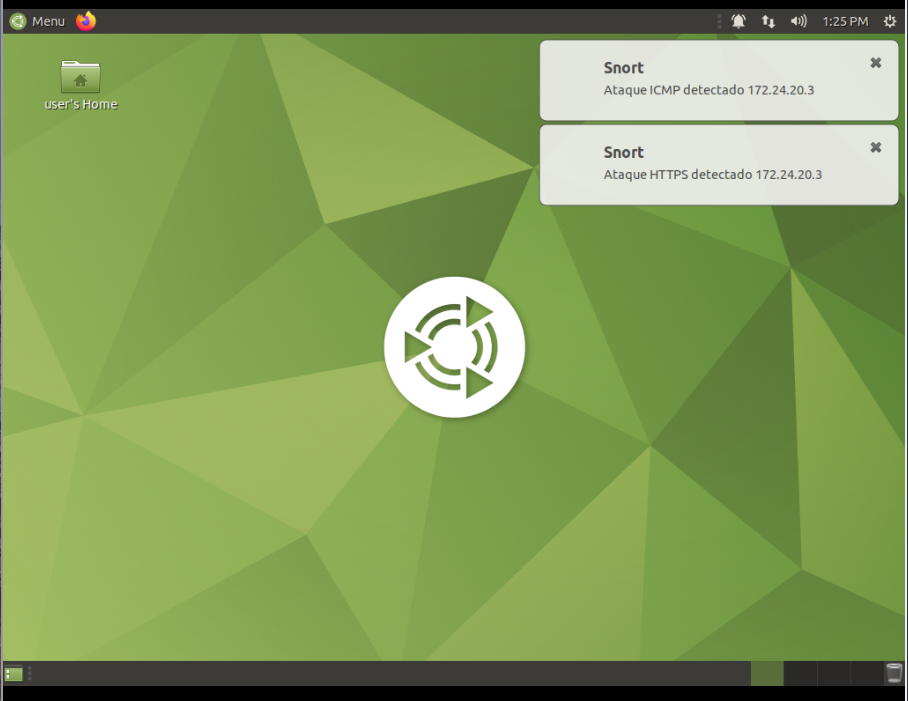
\includegraphics[width=1\linewidth]{fig/snort11.png}
    \caption{Notificações geradas a partir do monitoramento dos alertas do Snort}
    \label{fig:snort11}
\end{figure}

